% !TEX root = ../thesis-example.tex
%
\chapter{Background}
\label{sec:background}

\cleanchapterquote{
	\emph{visu|al|ize}, \ verb\\
	\begin{enumerate}
		\vspace{-3mm}
		\item to form a picture of somebody/something in your mind
		\vspace{-3mm}
		\item to make something visible to the eye
		\vspace{-2mm}
	\end{enumerate}
}{Oxford Advanced Learner's Dictionary}{}

\section{Visualization}
%introduce the general concept of perception, overview over the history, introduce the different facets of visualization as in my lecture
Forming an \SYN{all-encompassing} definition of visualization is a non-trivial task.
In 1987, when computer-aided visualization started to emerge, McCormick et al. \SYN{state} in \cite{McCormick:1987:DefinitionOfVisualization}: 
\begin{quote}
	``\emph{Visualization is a method of computing. It transforms the symbolic into the geometric, enabling researchers to observe their simulations and computations. Visualization offers a method for seeing the unseen.}''
\end{quote}
They assess two important things:
First, they identify the core \SYN{treat} of visualization, which is the mapping of abstract information into a graphical representation in order to make the information observable.
Second, they \SYN{nicely} phrase that effective visualization has the power to show information and relationships, which would not be observable from the raw data itself.
Since both the amount of data as well as the data density is continuously increasing, effective visualization becomes even more important as it also significantly increases the \SYN{speed and throughput} in which the human brain can process information.
Friedhoff and Kiley therefore write in \cite{Friedhoff:1990:eye}:
\begin{quote}
	``\emph{The standard argument to promote scientific visualization is that today's researchers must consume ever higher volumes of numbers that gush, as if from a fire hose, out of supercomputer simulations or high-powered scientific instruments. 
	If researchers try to read the data, usually presented as vast numeric matrices, they will take in the information at snail's pace. 
	If the information is rendered graphically, however, they can assimilate it at a much faster rate.}''
\end{quote}
One main reason of this \SYN{information inflation} is the \SYN{technical progress} leading to a constantly increasing amount of instrument data (e.g. resolution) and furthermore bringing up novel technologies providing new modalities. 
At the same time, today's \SYN{complete digital interconnection} makes information available even if it is physically elsewhere.
This sheer amount of available data is \SYN{opposed} to the limits of the human cognition.
The \SYN{science of} visualization provides effective tools to analyze, aggregate, reshape and present abstract information in a form facilitating its \SYN{comprehension} and possibly even allowing the observer to discover otherwise hidden \SYN{relationships, features}.
Good visualization exploits the power of human perception in order to reduce the observer's cognitive load.

With today's computational capabilities, the interaction aspect of visualization becomes more and more important, in particular with large amounts of data to process.
In order to explore the available data, understand it correctly and \SYN{pull the right conclusions} the user needs to be able to adapt the visualization to their needs.
With this requirement in mind, Shneiderman formulated his \emph{Information Seeking Mantra} in \cite{Shneiderman:1996:TheEyesHaveIt}:
\begin{quote}
	``\emph{There are many visual design guidelines but the basic principle might be summarized as the Visual Information Seeking Mantra:\\
		\hspace*{2em}Overview first, zoom and filter, then details-on-demand\\
		\hspace*{2em}Overview first, zoom and filter, then details-on-demand\\
		\hspace*{2em}Overview first, zoom and filter, then details-on-demand\\
		\hspace*{2em}Overview first, zoom and filter, then details-on-demand\\
		\hspace*{2em}Overview first, zoom and filter, then details-on-demand\\
		\hspace*{2em}Overview first, zoom and filter, then details-on-demand\\
		\hspace*{2em}Overview first, zoom and filter, then details-on-demand\\
		\hspace*{2em}Overview first, zoom and filter, then details-on-demand\\
		\hspace*{2em}Overview first, zoom and filter, then details-on-demand\\
		\hspace*{2em}Overview first, zoom and filter, then details-on-demand}''	
\end{quote}
\TODO{discuss more}

\subsection{Definition and Disambiguation}
\label{sec:background:vis:definition}
%Similar as in my lectures: 
%Present different definitions of visualization. 
%Then distinguish it from related fields of research, such as Computer Graphics, Image Processing, Computer Vision, Visual Analytics, etc. 
%Finally, introduce the classification of Information Visualization vs. Scientific Visualization.
The field of visualization is \SYN{closely} related to other research fields, such as computer graphics, image processing and computer vision.
However, each of these sciences has it's own part in the \III{visual taxonomy} \CN:
\begin{my_list_desc}
	\item[Computer Graphics]
		Both visualization and computer graphics deal with image synthesis the transformation of abstract data into graphical representations.
		However, while computer graphics deals with the technical and implementation aspects on how one can generate such pictures, visualization focuses on the data abstraction itself and which is its best visual representation for a given goal.
		Computer graphics targets efficient algorithms while visualization targets effectiveness to use.
	
	\item[Computer Vision]
		Visualization maps abstract information to visual representations.
		In computer vision one performs the inverse task and tries to interpret images in order to extract information from them.
	
	\item[Image Processing]
		The field of image processing is closely related to visualization and often performed in combination.
		However, the input and output data of image processing \SYN{remains} in the same domain since image processing maps data to data or images to images.
		In contrast, visualization maps data to images.
	
	\item[Perception]
		The \SYN{science of physiological perception} provides important insight into how the human visual system works.
		This knowledge can be used to create better visualization.
	
	\item[Augmented Reality] 
		\TODO{Augmented Reality...}
		Both visualization and AR use rendering techniques from Computer Graphics in order to generate their output.
		However, while visualization focuses on how to visualize abstract data by itself, augmented reality \SYN{investigates} how such visualizations can be integrated with \SYN{the real world} as good as possible.
\end{my_list_desc}

The visualization community distinguishes \emph{information visualization} from \emph{scientific visualization}.
Though it is certainly not a less scientific field of research, the former deals with the representation of abstract, often multi-modal $n$-dimensional data, which usually has no spatial domain by default.
In contrast, scientific visualization focuses on the representation of physical data, which has an inherent spatial and/or temporal reference and is of rather small (usually two to four) dimensionality.
Though mixed forms exists, these two classifications of visualization use different methods of visual representation.
Since this work is \SYN{on/about} medical visualization this thesis will focus on methods for scientific visualization.


\subsection{Goals and History of Visualization}
%Introduce the different abstract goals of visualization, such as to map, record, abstract, clarify, interact, communicate, etc.
%This is also a good place to present important historic milestones in visualization.
Though visualization as scientific research field has only emerged in the \SYN{last decades,last 30 years}, visualization techniques have been used ever since to store and transport information.
The extensive list on ``Milestones in the history of thematic cartography, statistical graphics, and data visualization'' \CN provides a detailed overview of the developments.

\begin{figure}[ht]
	\centering
	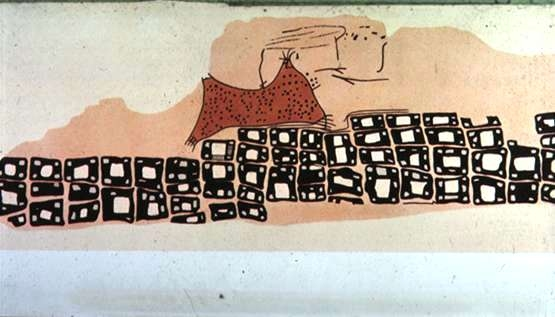
\includegraphics[width=0.75\linewidth]{figures/konya-town-map.jpg}
	\caption{Redrawing of the image found at the Çatalhöyük site depicting a map of a town, probably Çatalhöyük itself, from 6200 B.C. \cite{Web:KonyaTownMap}.}
	\label{fig:konya-town-map}
\end{figure}
%
One of the main goals of visualization is to provide an overview.
The oldest known map of a town is the drawing found at the Çatalhöyük size in Turkey and dated to 6200 B.C. 
Figure \ref{fig:konya-town-map} shows a reconstruction.
The Peutinger map, named after a 16th century German collector, is considered the first visualization showing a route map, to some extent comparable to today's subway maps (Figure \ref{fig:peutinger-map}).
The 34 centimeters by 7 meters large parchment depicts the whole Roman world of that time from Vienna, through Italy to Carthage.
Most probably intended to be used as a travel map, it does not show places and distances in scale but mentions the connections between places and how one has to travel.
The exact date of origin can not be determined but one estimates that the original cartographer lived in the fourth century \cite{Friendly:95:Milestones,Web:LiviusOrg:PeutingerMap}.
%
\begin{figure}[ht]
	\centering
	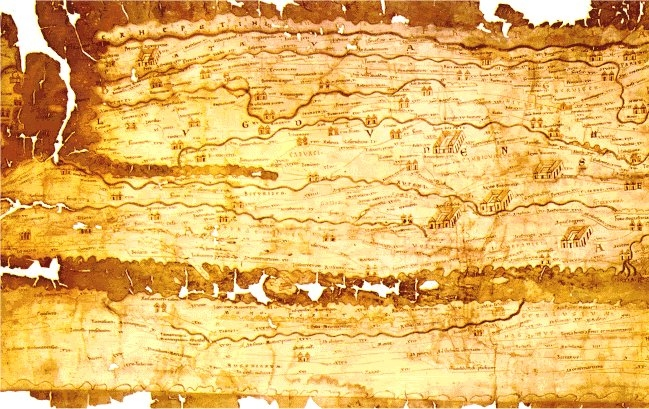
\includegraphics[width=0.75\linewidth]{figures/peutinger-map.jpg}
	\caption{First sheet of the Peutinger map showing the eastern part of Britain, Holland, Belgium, a part of France and the west of Morocco \cite{Web:LiviusOrg:PeutingerMap}.}
	\label{fig:peutinger-map}
\end{figure}

Another important goal of visualization is to record findings in order to \SYN{keep} the information and make it possible to \SYN{pass it to others}.
Impressive examples are the historic notebooks from Leonardo da Vinci in which he kept his findings of his scientific studies on a wide range of physical phenomena. 
His observational approach to science, in which he tried to understand them by highly detailed describing and depicting of each sample, lead to an incredible amount of scientific visualizations.
\SYN{Let alone} his planned book on the human anatomy ``\emph{De figura umana}'' was to contain 120 chapters recording his anatomical findings (cf. Figure \ref{fig:leonardo-drawings}) \cite{Capra:2013:LearningFromLeonardo}.
%
\begin{figure}[ht]
	\centering
	\subfloat[~The mechanisms of the hand.]{
		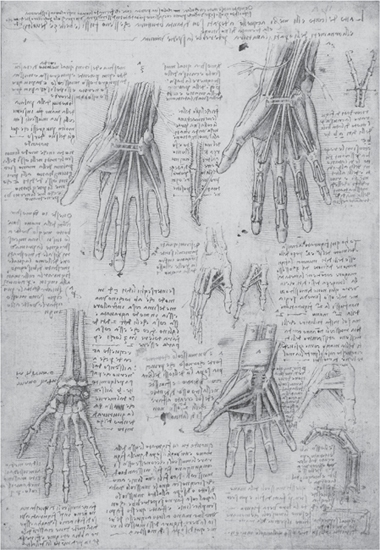
\includegraphics[height=7cm]{figures/leonardo-hand.jpg}
	}
	\qquad
	\subfloat[~Composite view of the internal organs of a woman’s body.]{
		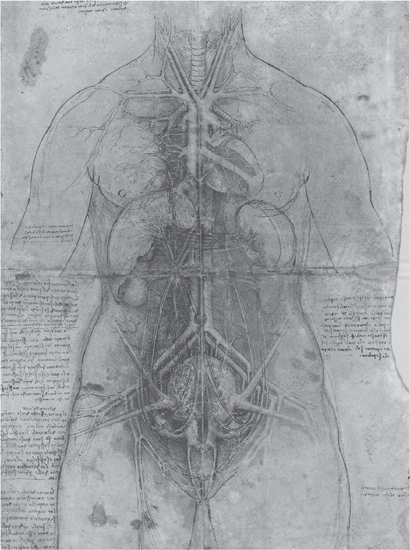
\includegraphics[height=7cm]{figures/leonardo-abdomen.jpg}
	}
	\caption{Examples of Leonardo da Vinci's recordings on his observations of the human anatomy \cite{Capra:2013:LearningFromLeonardo}.}
	\label{fig:leonardo-drawings}
\end{figure}

The power of abstraction allows visualization to tell a story \SYN{out of} complex data.
The map of Napoleon's Russian campaign of 1812 (cf. Figure \ref{fig:napoleons-march}), drawn in 1869 by Charles Minard, is considered as one of the most powerful visualizations in this regard.
Showing the number of soldiers over time and covered distance in relation to geographical \SYN{features} (e.g. rivers) and temperature, it succeeds in elegantly mapping this very heterogeneous and multi-dimensional data into a single image \cite{Tufte:1983:VisualDisplay,Chen:2010:InformationVisualization}.
%
\begin{figure}[ht]
	\centering
	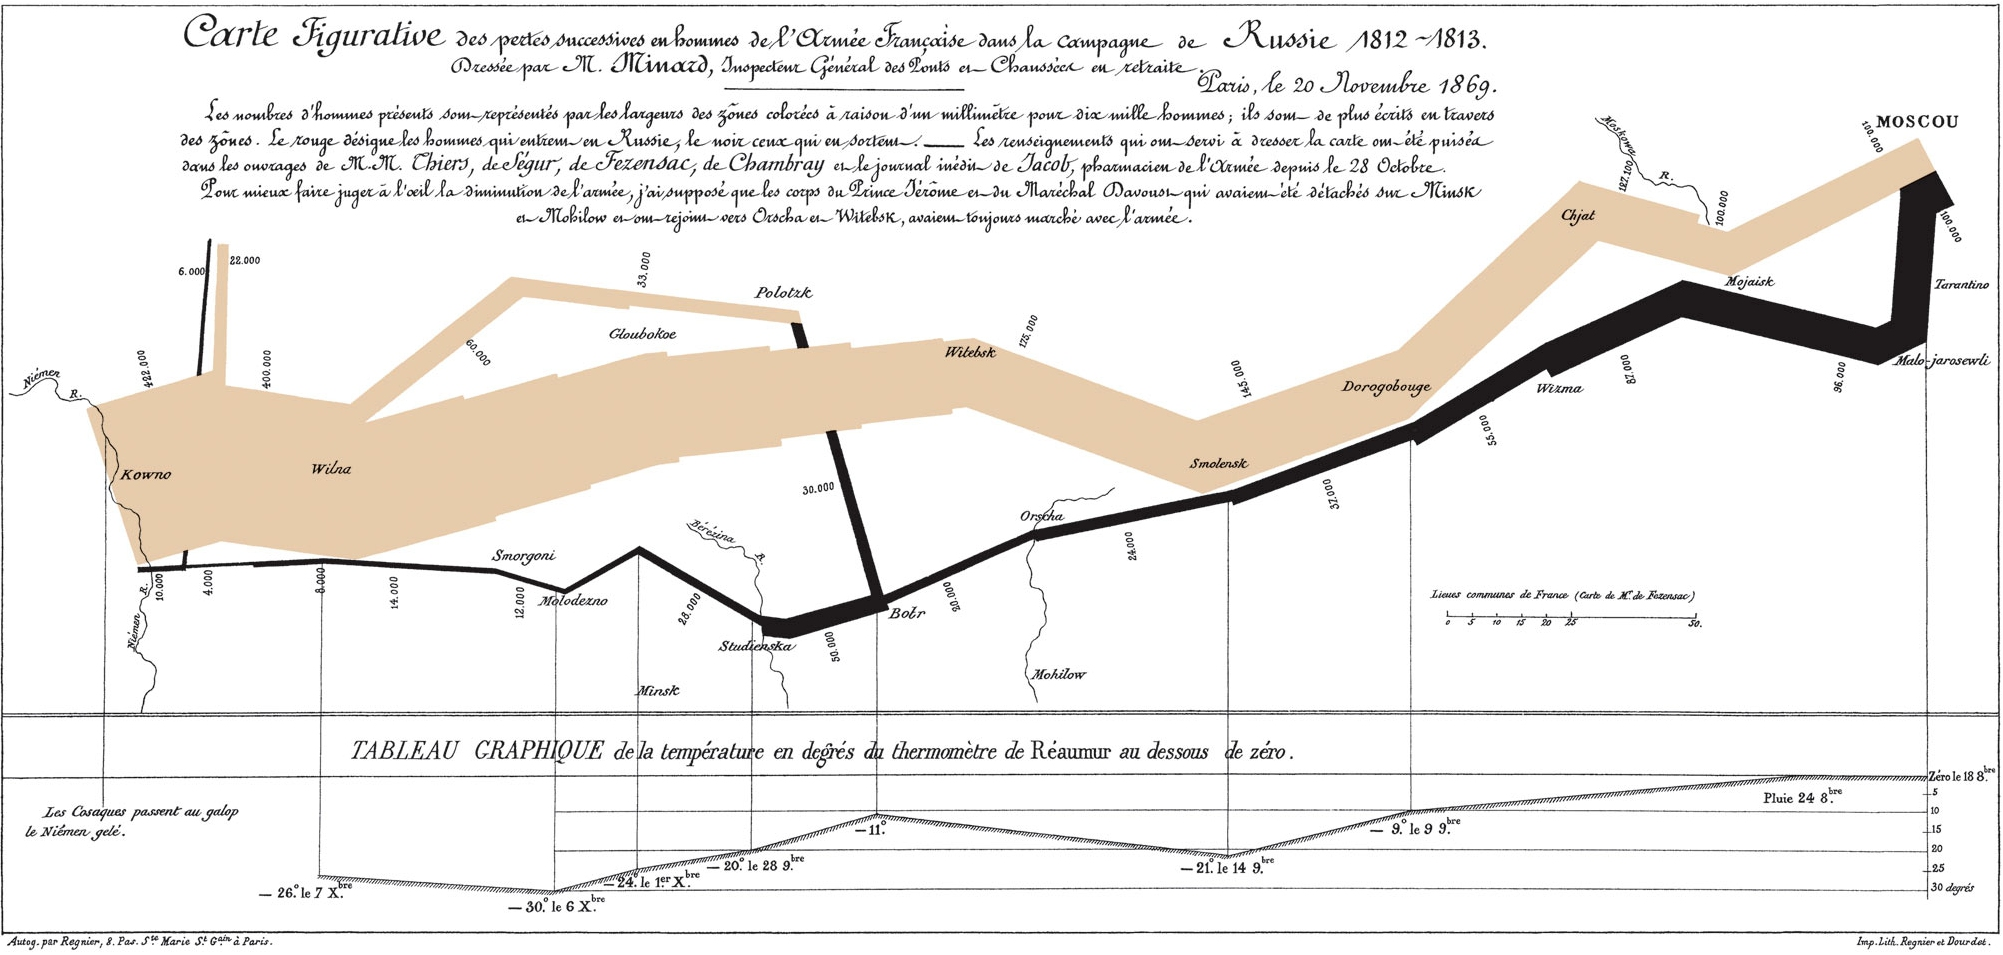
\includegraphics[width=0.75\linewidth]{figures/napoleons-march.jpg}
	\caption{Charles Minard's visualization of Napoleon's Russian campaign is considered as one of the most powerful exemplars of storytelling.}
	\label{fig:napoleons-march}
\end{figure}

Furthermore, carefully designed visualization allows to discover new facts and otherwise hidden relationships.
For instance, John Snow's dot map on the London cholera epidemic of 1854 (cf. Figure \ref{fig:cholera-map}), where he placed a dot on a London street map for each death, shows a clear clustering around a the Broad Street water pump.
This brought the English physician to the conclusion that the water of this particular well has to be contaminated \cite{Tufte:1997:VisualExplanations,Chen:2010:InformationVisualization}.
%
\begin{figure}[ht]
	\centering
	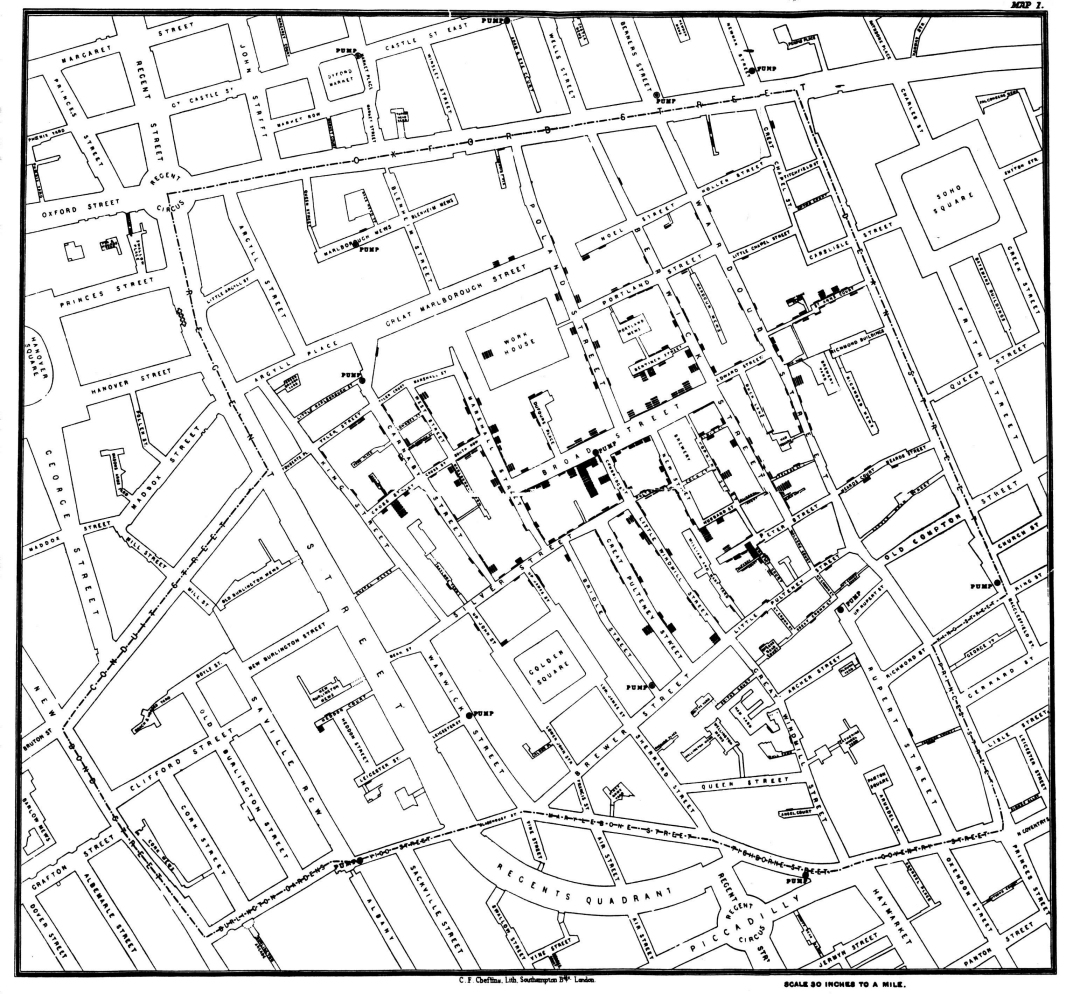
\includegraphics[width=0.75\linewidth]{figures/cholera-map.jpg}
	\caption{Charles Cheffins' lithography of John Snow's cholera epidemic map showing clusters around the Broad Street water pump. Each bar stands for one death during the London cholera epidemic of 1854.}
	\label{fig:cholera-map}
\end{figure}



\subsection{The Visualization Pipeline}
\label{sec:background:vis:vispipeline}

\CN~ formulate the \emph{visualization pipeline}, which \SYN{splits} the creation of visualizations into four steps (cf. Figure \ref{fig:vispipeline}).
As a first step, the information that should be visualized has to be gathered.
This can be done in different ways. 
Traditionally, raw data is measured using physical processes, such as X-ray attenuation, magnetic resonance or ultrasound in the case of medical imaging.
Alternative data sources can be simulation or modeling.
In the second step the acquired raw data has then to be processed, \SYN{such as} applying transformations, filtering, interpolation or deriving data otherwise.
This step usually falls into the field of signal- or image processing.
The third step of the visualization pipeline is mostly the actually visualization part of mapping the processed data into graphical representations.
This mapping relates to generating renderable data in terms of graphical primitives and assigning optical properties.
In the final step one uses computer graphics tools to render the visualization onto the screen.



\subsection{Data Characteristics}
\label{sec:Background:DataCharacteristics}
%I don't like the title of this subsection, I should think of a better one.
%Introduce the Information Seeking Mantra, the Visualization Pipeline (citation?), applications?
%Introduce different data characteristics and explain why they are important for visualization.
%At this point, I might also relate them to the special field of Medical Visualization, however, I'm currently not sure whether this makes sense at this point.
Effective visualization always needs to be tailored to fit to the individual characteristics of the input data.

\begin{my_list_desc}
	\item[Source]
		One main characteristic is the origin of the data.
		As already mentioned in Section \ref{sec:background:vis:vispipeline}, there exist three different data sources. 
		The input data can either be an \SYN{image} of the real world (through measuring), originate from theory (simulation) or \SYN{art,design} when originating from modeling \CN.
		Each of the three possible data sources has individual and different features and characteristics such as data credibility, distribution of uncertainty, noise, etc.
	
	\item[Domain]
		The second important data characteristic is the domain, for which one usually distinguishes four classes (cf. Table \ref{tbl:ListOfScales}).
		\emph{Nominal} data, sometimes also referred to as categorical data, can mathematically be described as a permutation group \cite{Stevens:1946:TheoryOfScales}.
		Since nominal data has no assigned ordering, the single comparison operation that can be applied is the test for equality.
		In cases where one can define an additional rank-ordering operation on the data domain, one speaks of \emph{ordinal} data, where the ordering measure can determine greater or less but does not allow for mathematical calculations.
		For instance, for two ordinal elements $a, b$ one can define that element $a$ is greater than $b$ but not that $a$ has twice the size of $b$.
		Finally, there is \emph{metric} data, which allows measuring the distance between two elements.
		This last class is often further split into continuous metric (real values) and discrete metric (distinct values) as in \CN or into interval scale and ratio scale as in \cite{Stevens:1946:TheoryOfScales}.
		The data domain significantly influences the design decisions when creating visualizations.
		For instance, when representing values through color, the employed color map has to be chosen carefully as described in Section \ref{sec:background:colorperception}.

	\item[Dimensionality]
		The third data characteristic is the dimensionality of each data element itself.
		Most data is formed of 1D scalar elements, such as Hounsfield units in CT volumes.
		However, other element dimensionalities appear as well, such as 3D vector data in flow or strain data, tensor data in Diffusion Tensor Imaging or even higher dimensions in multi-variate data.
		The data element dimensionality is one of the main constrains defining which visualization techniques are applicable.

	\item[Structure]
		Finally, the structure of the data forms an important data characteristic as well.
		One mainly distinguished scattered data (e.g. freehand SPECT events over time) from data aligned in a regular grid (e.g. reconstructed CT volume) \CN.
		The data structure \SYN{affects} which algorithms can be employed during the visualization pipeline since for instance scattered data does not exhibit implicit neighborhood information.
\end{my_list_desc}
\begin{table}[ht]
	\small
	\centering
	\begin{tabu} to 0.95\linewidth {>{\bfseries\centering}m{12mm} C C C}
		\toprule
		Scale    & \bfseries Comparison Operations      & \bfseries Mathematical Structure & \bfseries Permissible Statistics               \\
		\midrule
		Nomial   & Equality                             & Permutation group                & Number of cases, mode, contingency correlation \\
		Ordinal  & Greater/less                         & Isotonic group                   & Median, percentiles                            \\
		Interval & Equality of intervals or differences & General linear group             & Mean, standard deviation                       \\
		Ratio    & Equality of ratios                   & Similarity group                 & Coefficient of variation                       \\
		\bottomrule
	\end{tabu}
	
	\caption[List of scales (data domains) and their corresponding properties.]{List of scales (data domains) and their corresponding properties as described in \cite{Stevens:1946:TheoryOfScales}.}
	\label{tbl:ListOfScales}
\end{table}

\section{Medical Visualization}
%Not sure how to sectionize this, however I should have an in-depth discussion on general MedVis.
%The whole body of literature is extensive.
%Thus, I can only present a part of it.
%This could either be all MedVis techniques, which are relevant to my presented methods. 
%Alternatively, I can go through one of the data characteristics (i.e. dimensionality) and discuss MedVis techniques for each of the items (as I did in my lecture).
%One could also discuss multi-modal visualization.
\label{sec:Background:MedicalVisualization}
Due to the inherent spatial reference of most medical data, medical visualization is seen as a \SYN{sub part} of scientific visualization.
Even though McCormick's report on visualization in scientific computing from 1987 \cite{McCormick:1988:VisualizationInScientificComputing} is seen as the \SYN{birth,origin} of scientific visualization as a field of research, first examples of medical visualization have been published before.
In particular radiotherapy planning \SYN{axploited} the usage of computer-aided visualization systems.
First systems acquired patient contours with a mechanical digitizer, computed isodose distributions derived from multiple external beams and displayed both information \SYN{jointly} on an oscilloscope display \cite{Cox:1966:ProgrammedConsole,Holmes:1970:BeamTreatmentPlanning}.

Since the body of literature on medical visualization is by far too large to be completely covered within this work, the review in the thesis is limited to introducing the general concepts and provides detailed discussions only on works related to ultrasound processing and visualization.
For a complete and elaborate overview over the entire field of medical visualization, the reader is referred to the book of Preim and Botha \cite{Preim:2013:VisualComputingForMedicine}.


\subsection{Imaging Modalities}
\label{sec:background:imaging-modalities}
%discuss the main medical imaging modalities

Today's clinicians have a broad range of imaging modalities at their hands.
Since each modality has certain advantages and disadvantages they individually \SYN{excell} for certain applications.
Furthermore, one distinguishes between imaging modalities that show the underlying anatomy and functional modalities that show the \SYN{metabolism, meta-something} of the body.

\subsubsection{Fluoroscopy}
The oldest medical imaging modality is fluoroscopy and goes back to the discovery of X-Rays by Wilhelm Conrad Röntgen in the late 19th century, which he named after the unknown variable $x$ \cite{Roentgen:1898:NeueArtStrahlen}.
Today, the general setup of a fluoroscope consists of the X-Ray source, usually formed by a tube emitting X-Ray photons of a specific intensity, and the X-Ray detector.
The two are placed at opposing sides of the target anatomy, so that the rays can travel through the tissue.
The resulting image shows the originally emitted energy minus the attenuation based on absorption and scattering within the tissue.

Fluoroscopy is frequently used in clinical practice due to being cost-effective and real-time capable.
In particular, bones and other high-attenuation structures such as surgical tools show good image contrast, while soft tissue differences are hard to \SYN{show}.
Furthermore, the 2D projection show the integrated attenuation along the entire ray so that it is hard to determine positional relationships, particularly in depth.
The major drawback of fluoroscopy is the usage of ionizing radiation, which has the potential impair the genetic material of both the patient and clinical staff.
From the visualization \SYN{perspective/point of view}, X-Ray images are thus characterized by 1D metric data (intensities), arranged in a regular, 2D rectilinear grid.
Traditionally, these intensities are displayed as gray-scale images \II.



\subsubsection{X-Ray Computed Tomography}
In order to overcome the limitation of X-Ray only showing 2D projections, clinicians often take multiple X-Rays from different viewing directions.
X-Ray Computed Tomography (CT), originally proposed by Godfrey Hounsfield \cite{Hounsfield:1973:ComputedTomography}, performs this in a systematic manner by rotating source and detector axially around the object by at least 180°.
Tomographic reconstruction algorithms, such as the filtered backprojection \CN, then reconstruct a volumetric representation of the scanned anatomy, where each element describes the local attenuation coefficient.

While the drawback of using ionizing radiation remains, CT offers a significantly increased scanning resolution compared to fluoroscopy and further allows to show arbitrary cross-sectional images of the anatomy, so that pathologies can be exactly located \II.
Modern multi-slice CT scanners even allow the acquisition of volumetric images in real-time in order to study dynamic processes over time.
Gating techniques thereby reduce the amount of artifacts when scanning periodically moving anatomy such as the heart.
The domain and dimensionality of CT data are still 1D intensities but they structured in a 3D grid, possibly with an additional time domain.
In order to make CT scans better comparable, their intensities are normalized into Hounsfield Units (HU), which map water to zero and air to $-1000$.
Hence, given an attenuation coefficient $\mu$, the corresponding Hounsfild Unit is defined by
\begin{equation}
	\label{eq:background:HU}
	HU = \frac{\mu - \mu_{\text{Water}}}{\mu_{\text{Water}}} \cdot 1000,
\end{equation}
where $\mu_{\text{Water}}$ is the attenuation coefficient of water.



\subsubsection{Magnetic Resonance Imaging}
Magnetic Resonance Imaging (MRI) is based on physical properties of tissue in presence of a magnetic field.
A strong, uniform magnetic field is applied so that the protons of the hydrogen atoms in the anatomy are aligned while spinning arbitrarily around the axis of the field.
An additional pulsating magnetic field let's all protons precessing at the given frequency resonate and precess in the plane orthogonal to the magnetic field.
When the pulse is switched off, the protons return to their equilibrium orientation while emitting electromagnetic signals, which are detected by the scanner.
Since the concentration of protons is tissue-specific, the relaxation time allows to draw conclusions \SYN{about,on} the tissue type and one can reconstruct a volumetric representation of the anatomy.

So far, a plethora of MRI protocols have been developed, which allow for both anatomical and functional imaging.
For instance, the traditional $T_1$ and $T_2$ weighted images \CN~ show 1D intensities with excellent soft-tissue contrast.
The more complex protocol of diffusion-weighted imaging allows to measure the amount of diffusion along certain directions.
In Diffusion Tensor Imaging this information is reconstructed into 3D volumes of second-rank tensors modeling the distribution of diffusion present in the anatomy, so that the dimensionality of each data element is six.
Compared to CT, MRI has the huge advantage of being radiation-free and showing better soft-tissue contrast while providing a comparable resolution and signal-to-noise ratio.
However, acquisition times are much longer and the general costs are considered higher.
Furthermore, the inherent strong magnetic field significantly complicates the deployment for applications in the operating room.



\subsubsection{Ultrasound}
Ultrasound imaging (US) uses high frequency sound waves, which are emitted from a transducer into the anatomy.
In order to improve the transmission, a special ultrasound gel is used as coupling in between.
The ultrasound travels as \SYN{longitudinal} waves through the patient's body and gets partially scattered and reflected at tissue interfaces of different acoustic impedance.
When the reflected waves get back to the transducer, their time delay is recorded as scan line data.
A post-processing pipeline converts the scan line data into B-mode images showing intensities in a regular 2D grid depicting the echo in the corresponding image plane.
Different imaging modes allow to measure additional information such as flow velocities (Doppler US) or elasticity (Elastography US) \II \CN.
Special matrix transducers allow to record 3D B-mode volumes at real-time.
Tracking systems allow to acquire tracked ultrasound sweeps, a series of 2D B-mode images, where each image is arbitrarily oriented in space, significantly \SYN{extending} the data structure.
Ultrasound compounding techniques allow to reconstruct this scattered, unstructured data back into a regular 3D volumetric representation.

Ultrasound is a widely used imaging modality mainly due to being very cost-effective, real-time capable and being radiation-free.
Furthermore, ultrasound machines have a very small footprint and are thus mobile and can be specialized for many different clinical applications \parencite{Noble:2011:Ultrasound}.
However, ultrasound images are very \SYN{hard} to interpret, since the ultrasound image formation process is very complex and the resulting images often exhibit low contrast and a low signal-to-noise ratio.
A particular challenge for visualization is the highly non-uniform meaning of B-mode intensities.
In contrast to CT Hounsfield units or most MRI intensities, ultrasound intensities do not form an interval scale (cf. Section \ref{sec:Background:DataCharacteristics}) and can not necessarily be compared within the same image.
A more thorough discussion of Ultrasound imaging and its visualization can be found in Section \ref{sec:Background:UltrasoundVisualization}.


\subsubsection{Nuclear Imaging}
Nuclear imaging allows to show functional processes such as metabolic processes.
Therefore, a special radioactive tracer substance is injected into the body, which accumulates in the target anatomy where it decays over time.
Positron Emission Tomography (PET) detects the gamma photons emitted by the annihilated positrons using a dense circular detector setup.
Single Photon Emission Computed Tomography (SPECT) use 2D gamma cameras, which are rotated around the target anatomy similar to the CT setup.
Both modalities reconstruct 3D volumetric images but with significantly lower resolution that CT or MRI.
Since they only exhibit functional information they are often combined with anatomical modalities, such as CT.
As of today, there exist fully integrated PET/CT, PET/MRI, and SPECT/CT scanners \CN.

In order to avoid the large footprint of conventional SPECT scanners, recent works introduced freehand SPECT acquisitions using tracked Gamma cameras \CN.
In this case the data structure changes, since it is no longer formed by a regular grid but a series of 2D projections arbitrarily scattered in 3D space.




\subsection{Basic Visualization Techniques for Medical Data}
As discussed in the previous section, most imaging modalities store their acquired data in a structured representation, usually a regular, rectilinear 2D or 3D grid.
This simplifies the subsequent visualization techniques since the spatial information (i.e. the position of each sample) is inherently encoded within the data.
However, depending on the \SYN{remaining} data characteristics of domain and dimensionality there are different visualization techniques applicable.


\subsubsection{Visualization of Scalar Data}
Most medical data is formed of discrete metric scalar data stored in a 2D or 3D regular grid.
Thus, there is a wide range of visualization techniques available.

\paragraph{Slice Rendering}
The traditional technique for displaying scalar medical data is slice rendering.
In case 2D data, such as radiographs or 2D B-mode ultrasound, displaying the image on the 2D screen is straight-forward.
For \SYN{tomographic/volumetric} data however, different methods exist to extract a 2D slice.
The classic approach is to display a slice, which is aligned orthogonally to one of the three main axes.
Actually, early CT scanners did not reconstruct complete 3D volumes but stacks of axial 2D slices \CN.
Even today, many clinicians still just cycle through this stack of axial slices and build the 3D model in their head as they have been trained to do so \CN.

However, often the target anatomy is not aligned well with the three main axes so that important information can not be displayed in a single slice.
Therefore, multi-planar reformations (MPR) allow to define an arbitrary plane through the 3D volume, which will then be resampled at the intersection \II\CN.
Displaying such 2D views is natively supported by most of today's GPUs \CN.

Curved planar reformations (CPR) go even further and project a \SYN{bent, curved} cut plane through the volume into a 2D image.
Kanitsar et al. propose to use this technique for vessel visualization since it allows for easier recognition of vessel wall abnormalities (cf. Figure \ref{fig:background:CPR}) \cite{Kanitsar:2002:CPR,Kanitsar:2003:CPR}.
Williams et al. adapt this technique so that it can also be used with larger tubular structures such as the trachea and the colon \cite{Williams:2008:VirtualColonoscopy}.
Kretschmer et al. generalize this approach and introduce Anatomy-driven Reformation.
Their straightening and unfolding of bone structures such as the rib cage allows clinicians to easier spot small bone lesions (cf. Figure \ref{fig:background:ADR}) \cite{Kretschmer:2014:ADR}.

\begin{figure}[ht]
	\centering
	\subfloat[~Example of a color coded curved planar reformation showing the aorta and surrounding vasculature as in \cite{Kanitsar:2003:CPR}.]{
		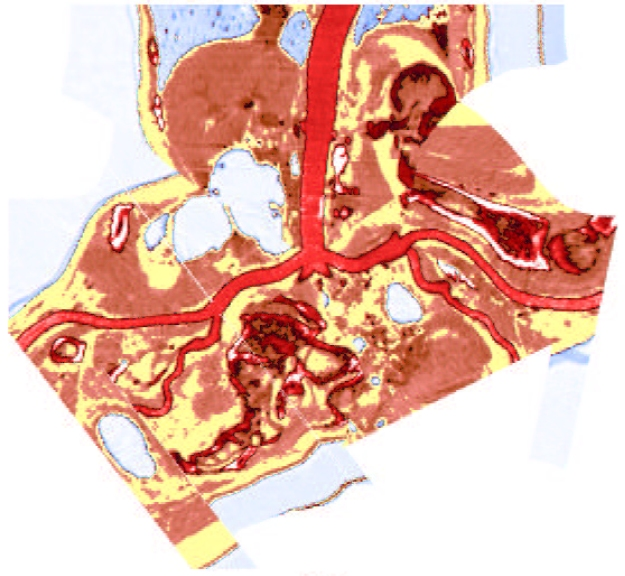
\includegraphics[height=4.5cm]{figures/background/cpr.jpg}
		\label{fig:background:CPR}
	}
	\qquad
	\subfloat[~Example of Anatomy Driven Reformation of the rib cage as shown in \cite{Kretschmer:2014:ADR}.]{
		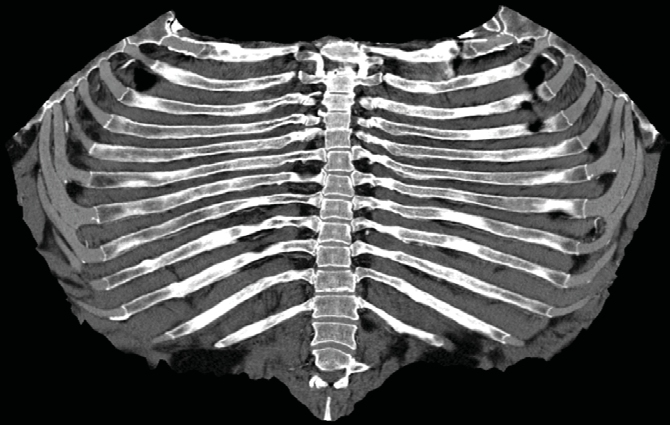
\includegraphics[height=4.5cm]{figures/background/adr.jpg}
		\label{fig:background:ADR}
	}
	\caption{Illustration of advanced reformation techniques embedding non-flat surfaces into a 2D image.}
	\label{fig:background:non-linear-reformations}
\end{figure}


\paragraph{Volume Rendering}
Even advanced reformations are limited in the amount of information that they can show and require the clinician to build the complex three-dimensional model of the anatomy in their mind.
Therefore, volume rendering technique allow to display the volumetric information in an \SYN{intuitive} way.
Technically, one distinguishes \emph{indirect} volume rendering from \emph{direct} volume rendering.
The former techniques first extract a geometry representation from the volumetric image data, which can then be rendered using classic computer graphics rendering pipeline.
The intermediate geometry can be either defined through the results of segmentation algorithms or as isosurfaces of a certain intensity.
The classic algorithm for isosurface extraction is still the Marching Cubes algorithm originally proposed by Lorensen and Cline \cite{Lorensen:1987:MarchingCubes}.
However, many more algorithms exist, which are often specialized for individual applications \cite{Livnat:2005:IsosurfaceExtraction}.

With the increasing \SYN{power} of graphics processing hardware, direct volume rendering techniques became feasible to be implemented in real-time.
Instead of extracting an intermediate geometry representation, those algorithms operate directly on the volume data and project it onto the 2D viewport by simulating the physics of light transport through ray casting \cite{Engel:2006:VolumeGraphics}.
Many of today's implementations are still based on the image order approach as proposed by Krüger and Westermann, which can be easily implemented in modern GPUs \cite{Kruger:2003:RayCasting}.
A set of virtual rays is casted from the camera through the viewport plane into the volume.
These rays are then traversed at a \SYN{certain, given} sampling interval and for each sample the local image intensity is looked up and mapped to optical properties, which are eventually integrated along each ray using a given compositing scheme as illustrated in Figure \ref{fig:background:ray-casting-scheme}.


For traditional photo-realistic rendering, one often approximates the physics of light transport with the emission-absorption model leading to the Volume Rendering Integral where the intensity $I$ at sample $s$ is given by
\begin{equation}
	\label{eq:VolumeRenderingIntegral}
	\begin{split}
		I(s)			&= 	I(s_0) \cdot e^{-\tau(s_0, s)} \ + \ \int_{s_0}^{s} q(\tilde{s}) \cdot e^{-\tau(\tilde{s}, s)} d\tilde{s}, \\	
		\tau(s_1, s_2) 	&=	\int_{s_1}^{s_2} \kappa(s) ds,
	\end{split}	
\end{equation}
with $q(s)$ being the emission coefficient and $\kappa(s)$ being the absorption coefficient for sample $s$ \cite{Max:1995:VolumeRenderingIntegral}.
This integral can be efficiently computed in an incremental scheme running either front-to-back or back-to-front.
Simpler compositing schemes, such as Maximum Intensity Projection (MIP) or Maximum Intensity Difference Accumulation (MIDA) \cite{Bruckner:2009:MIDA} are often used for visualizing vasculature or other high-contrast anatomy.
Digitally Reconstructed Radiograph (DRR) compositing allows to simulate fluoroscopy images from CT \cite{Metz:2005:DRR, Milickovic:2000:DRR}.
In the recent years, direct volume rendering techniques have been continuously improved in order to yield a more photo-realistic appearance through sophisticated global illumination models \cite{Lindemann:2011:IlluminationSurvey, Joensson:2014:IlluminationSurvey}, improve depth perception \cite{Svakhine:2009:DepthEnhancing, Kersten-Oertel:2014:DepthEnhancing}, and support even extensively large data sets through out-of-core rendering \cite{Crassin:2009:GigaVoxels,Crassin:2011:GigaVoxels}.


\paragraph{Classification}
One important step during the visualization of scalar data is the mapping of the scalar values to optical properties, such as color and transparency.
This step of defining the look of the data is referred to as classification and usually performed through transfer functions.
According to the introduced emission-absorption model (cf. Equation \ref{eq:VolumeRenderingIntegral}), a \SYN{simple} 1D transfer function defines an emission coefficient in terms of color (RGB) and an absorption coefficient in terms of opacity for each value of the input domain (usually scalar intensities).
Traditional transfer function editors allow to define such transfer functions by defining key/support points in a 2D graph mapping intensity to the horizontal axis and opacity to the vertical axis.
To provide a reference to the classified data set, a histogram of the intensity distribution is plotted in the background.
Examples of such a transfer function editor are shown in Figure \ref{fig:background:1dtf}).

\begin{figure}[ht]
	\centering
	\subfloat[]{
		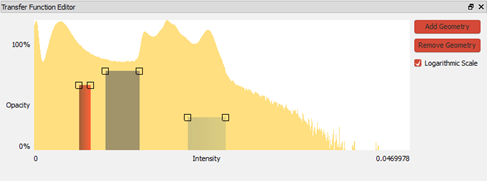
\includegraphics[height=3.25cm]{figures/background/tf1-editor.png}
		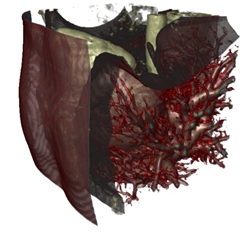
\includegraphics[height=3.25cm]{figures/background/tf1-result.jpg}
	}
	\\
	\subfloat[]{
		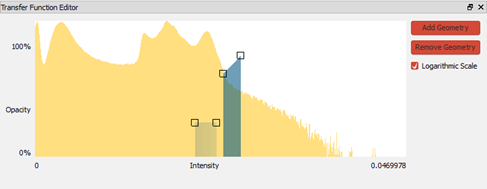
\includegraphics[height=3.25cm]{figures/background/tf2-editor.png}
		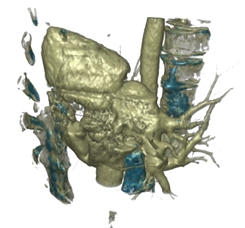
\includegraphics[height=3.25cm]{figures/background/tf2-result.jpg}
	}
	\caption{Examples of simple 1D transfer functions. \TODO{new images!}}
	\label{fig:background:1dtf}
\end{figure}

A standard CT data set usually allows for distinguishing different tissue types solely based on the Hounsfield units.
Thus, a 1D transfer function is sufficient to yield high quality visual results.
However, in contrast CT, some MRI sequences or ultrasound images the scalar intensities are ambiguous with respect to the tissue type so that advanced classification methods are required.
One solution is to increase the input domain and use multi-dimensional transfer functions as originally introduced by Levoy \cite{Levoy:1988:VolumeSurfaces}.
Often gradient magnitude is used as a second input dimension for the transfer function, which allows for a more precise extraction of certain tissue types.
%However, designing multi-dimensional transfer functions is a tedious and unintuitive task.
%Different approaches exists to facilitate this process.
Kniss et al. propose a set of direct manipulation widgets to define three-dimensional transfer functions based scalar intensity, gradient magnitude, and a second derivative measure \cite{Kniss:2002:MultidimensionalTf}.
Sereda et al. use LH histograms to identify tissue interfaces.
Plotting the LH space into a joint histogram reveals clusters for the different tissue types present in the data and allows for an easy definition of the transfer function through 2D geometric primitives \cite{Sereda:2006:LhHistograms}.
Another approach is to extract local shape information from the data and use this for advanced classification of the data \cite{Prassni:2010:ShapeBasedTf}.

Though multi-dimensional transfer function may yield more distinctly segmented visualization, their setup is often highly unintuitive.
Especially non-expert users struggle with mapping the complex parameter domain to semantic features for visualization, which makes such techniques \SYN{non-suitable} for clinical practice \cite{Salama:2006:SemanticTf}.
Different approaches exist to facilitate the process.
Stroke-based techniques let the user delineate in image space both structures that should be shown and structures that should be hidden, which are eventually mapped back to transfer function space.
Thereby, the frequent focus switch between the transfer function editor and the image data can be avoided \cite{Tzeng:2003:NovelInterface, Ropinski:2008:StrokeBasedTf}.
Another approach are data-driven techniques to (semi-) automatically generate presets based on clustering or statistical analysis \cite{RezkSalama:2000:AutomaticAdjustment, Patel:2009:MomentCurves}.
Introducing a semantic layer into the definition of transfer functions can make their setup more intuitive.
Therefore, Rezk-Salama et al. propose to use principal component analysis to map a small set of semantic parameters to the potentially large transfer function parameter space and claim that this can be learned from clinicians \cite{Salama:2006:SemanticTf}.
A different approach is the work of Rautek et al. who implement a fuzzy logic evaluation of the semantic descriptions on the GPU and combine it with interaction-dependent rendering \cite{Rautek:2008:SemanticsForIllustrativeVr}.
A very recently proposed technique combining the idea of design galleries \cite{Marks:1997:DesignGalleries} with modern touch interaction are dynamic galleries presented by Jönsson et al., which allow also novice users to intuitively explore volumetric data sets (cf. Figure \ref{fig:background:joensson-dynamicgalleries}) \cite{Jonsson:2016:DynamicGalleries}.
\begin{figure}[ht]
	\centering
	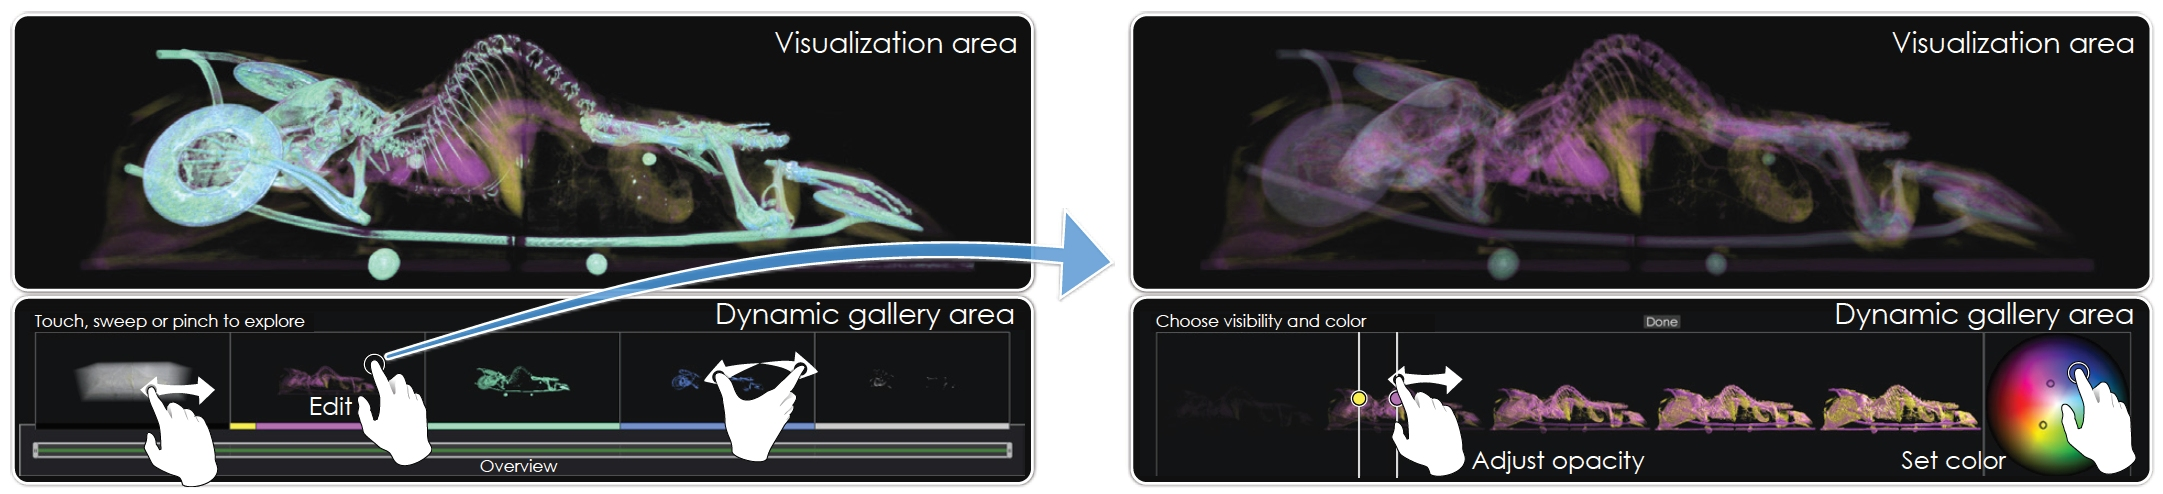
\includegraphics[width=0.9\linewidth]{figures/background/joensson-dynamicgalleries.jpg}
	\caption{
		Dynamic galleries as proposed by Jönsson et al. allow novice users to explore large volumetric data sets through intuitive touch interaction. Image from \cite{Jonsson:2016:DynamicGalleries}.
	}
	\label{fig:background:joensson-dynamicgalleries}
\end{figure}



\subsubsection{Visualization of High-dimensional Medical Data}
Not all medical data is formed solely by a scalar field.
Special imaging protocols allow to generate high-dimensional images, such as vector- and tensor fields.
Furthermore, there is often an additional time domain present.

\paragraph{Vector Data}
In vector fields, each element is formed by a (usually three-dimensional) vector.
Such data mainly occurs in flow applications such as the visualization of motion of fluids (e.g. blood), geometric boundary conditions, or deformation-/strain fields.
Typical visualization strategies include the display of arrow geometry, characteristic lines and dynamic particle simulations.

\begin{figure}[ht]
	\centering
	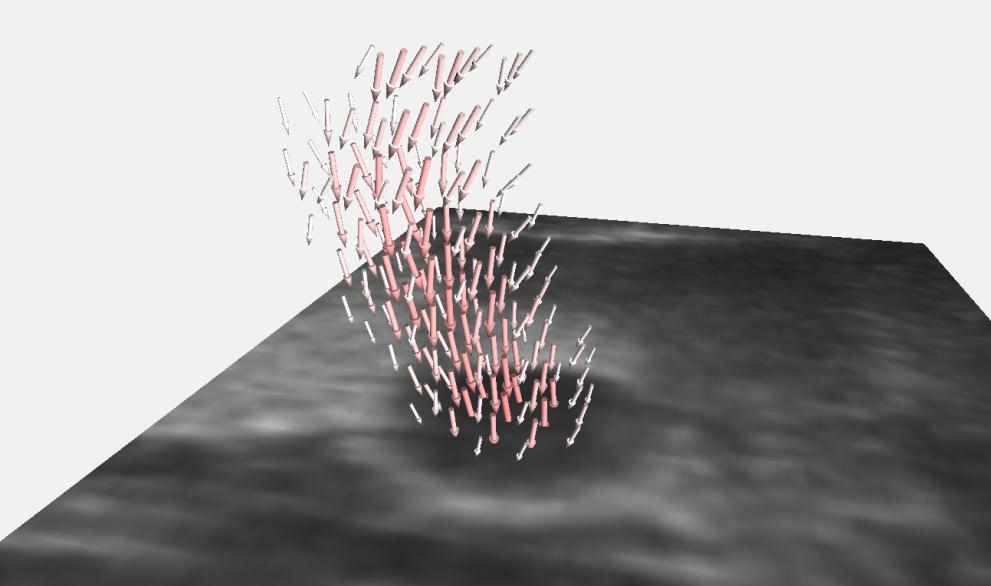
\includegraphics[width=0.75\linewidth]{figures/background/arrow-rendering.jpg}
	\caption{
		Arrow glyph rendering of the blood flow in the carotid artery reconstructed from tracked Doppler ultrasound data.
	}
	\label{fig:background:arrow-rendering}
\end{figure}
Direct techniques such as mapping the vector field to arrow glyphs (cf. Figure \ref{fig:background:arrow-rendering}) are the most straight-forward way of displaying such data and are often combined with color coding additional measures such as the gradient magnitude.
While they are rather simple to implement and can show direction, magnitude and vorticity of the vector field, they are usually hard to read since the dense geometry leads to occlusion and visual cluttering.
Dynamic particle visualizations simulate the behavior of particles in the flow field over time.
Since the user does not need to track single particles but rather observes general flow patterns they can provide a good overview over the properties of the flow field.
When combined with an interactive probing technique, this technique allows also for detailed examination of specific regions of interest \cite{VanPelt:2011:InteractiveProbing}.

Characteristic lines, such as streamlines, pathlines and streaklines, allow to observe the behavior of the particle flow over time in a single static image.
Streamlines only consider a static vector field an propagate a massless particle along the flow.
Thus, the resulting line is always tangential to the vector field.
Pathlines extend this concept to dynamic vector fields.
Streaklines depict the trace of dye that is constantly released into the flow at a fixed position.
Thus, they connect all particles that passed through a certain position.
Figure \ref{fig:background:characteristic-lines} illustrates the difference between these three types of characteristic lines.
\begin{figure}[ht]
	\centering
	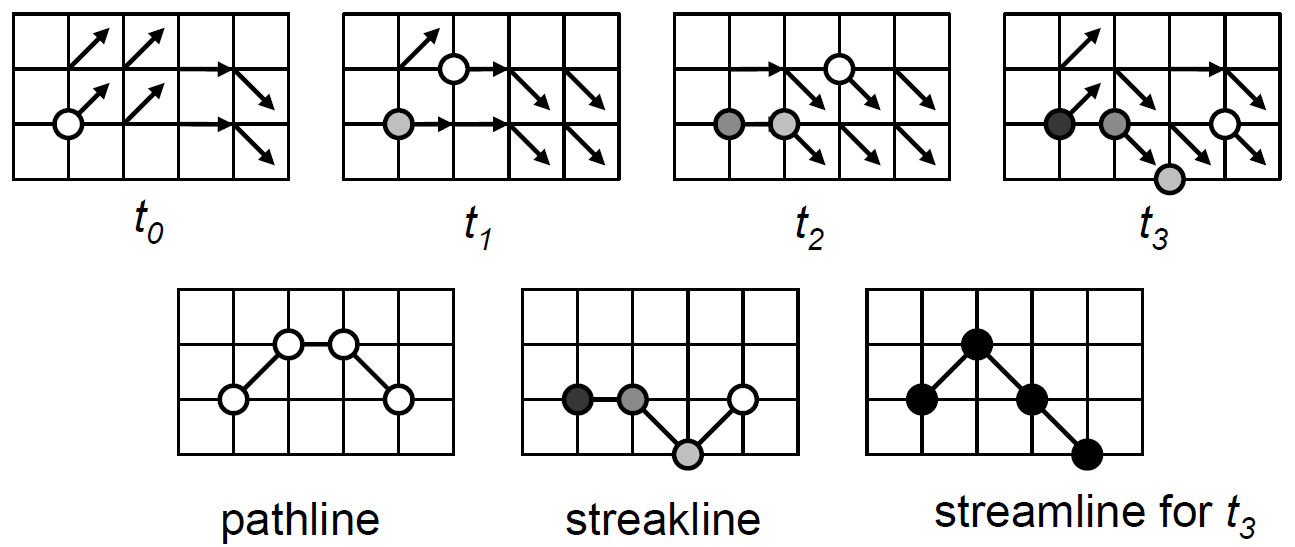
\includegraphics[width=0.75\linewidth]{figures/background/characteristic-lines.png}
	\caption{
		Comparison of streamlines, pathlines, and streaklines. 
		In a steady flow field, all three are identical.
		\TODO{redo this in TikZ}
	}
	\label{fig:background:characteristic-lines}
\end{figure}

Recent works on medical flow visualization combine these techniques with illustrative focus-and-context rendering techniques of the surrounding anatomy in order to provide a highly integrated result that allows the clinician to assess many different aspects in the data (cf. Figure \ref{fig:background:lawonn-flow}) \cite{VanPelt:2010:StylisticFlowVis, Gasteiger:2011:FlowLens, Lawonn:2016:BloodFlowWallThickness}.
\begin{figure}[ht]
	\centering
	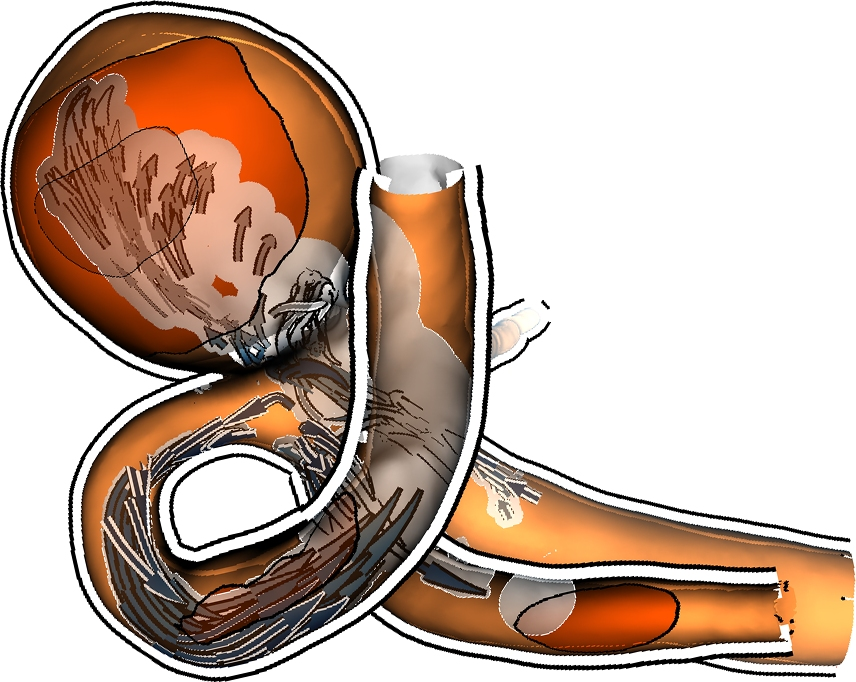
\includegraphics[height=4.5cm]{figures/background/lawonn-flow2.jpg}
	\quad
	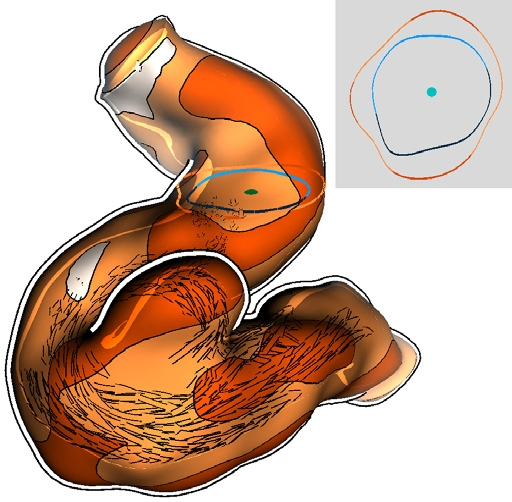
\includegraphics[height=4.5cm]{figures/background/lawonn-flow1.jpg}
	\caption{
		Examples of state-of the art flow visualization for vessels combined with a wall thickness estimation as presented by Lawonn et al. Images from \cite{Lawonn:2016:BloodFlowWallThickness}.
	}
	\label{fig:background:lawonn-flow}
\end{figure}

\paragraph{Tensor Data}
The mathematical tensor, a generalization of the concepts of scalars and vectors, is a geometric object describing linear relations.
In the context of medical visualization, the most common form is the diffusion tensor 
\begin{equation}
	D = \begin{pmatrix}
			D_{xx}	&	D_{xy}	& D_{xz} \\
			D_{yx}	&	D_{yy}	& D_{yz} \\
			D_{zx}	&	D_{zy}	& D_{zz}
		\end{pmatrix}
\end{equation}
used to model the amount of water diffusion in tissue, which can be measured by diffusion-weighted MRI \cite{Cercignani:2001:DWMRI, Westin:2002:DTMRI}.
In this diffusion tensor $D_{xx}$, $D_{yy}$ and $D_{zz}$ represent the amount of diffusion along the three main axes.
The other six off-diagonal values represent the correlation between the corresponding two perpendicular axes.

\begin{figure}[ht]
	\centering
	\subfloat[~Slice rendering of the fractional anisotropy of a DTI scan of a human brain. The cross-shaped red region in the center represents the corpus callosum, where a high density of fiber bundles is present.]{
		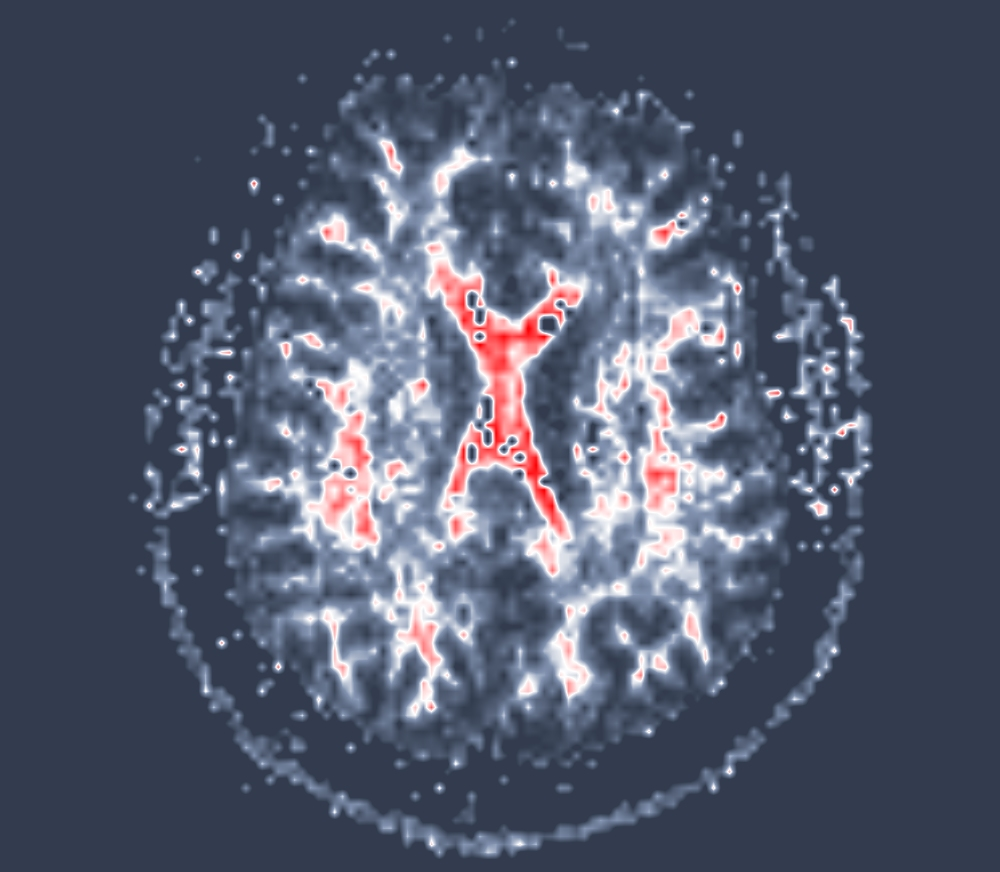
\includegraphics[height=6cm]{figures/background/dti-slicefa.jpg}
		\label{fig:background:dti-slicefa}
	}
	\quad
	\subfloat[~Streamtube rendering of the pyramidal tract reconstructed from DTI. Fiber visualization can depict global connectivity within the anatomy.]{
		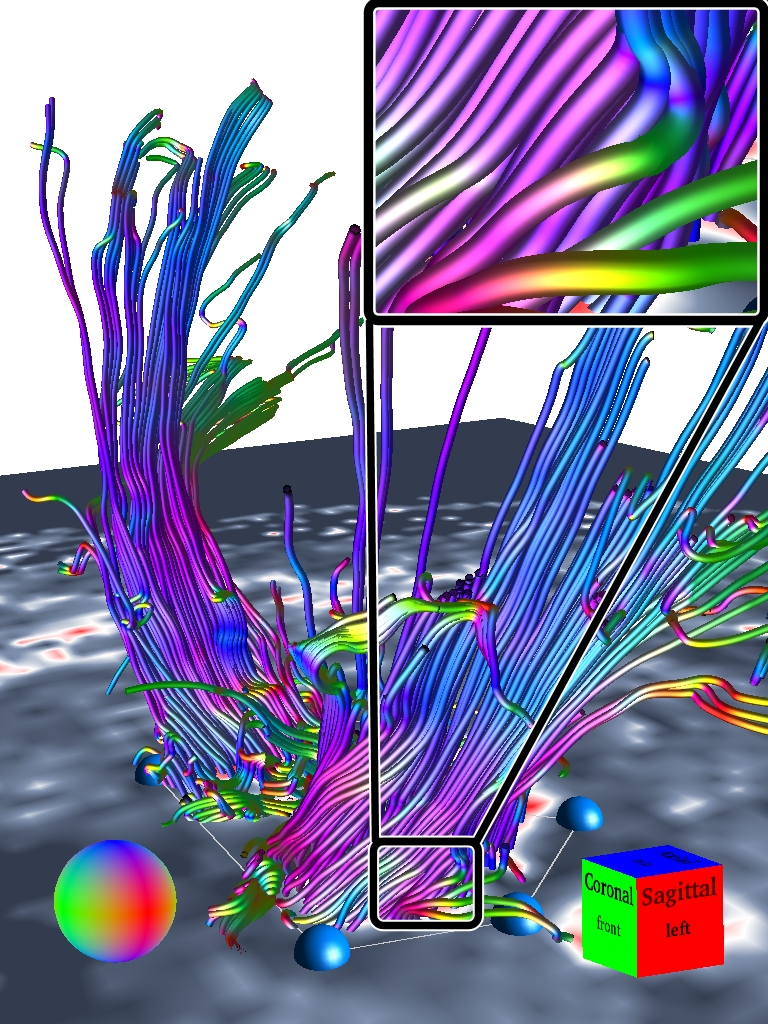
\includegraphics[height=6cm]{figures/background/dti-fibers.jpg}
		\label{fig:background:dti-fibers}
	}
	\caption{
		Examples of standard diffusion tensor visualization techniques. Both images show a DTI scan of a human brain.
	}
	\label{fig:background:dti-techniques}
\end{figure}

Traditional approaches to visualize this high-dimensional data use dimensionality reduction.
Various anisotropy measures (e.g. trace, fractional anisotropy, etc.) can be used to describe certain features of the diffusion tensor in scalar values \cite{Basser:2011:DTI, Westin:2002:DTMRI}.
The resulting scalar field can then be rendered using standard slice-based and volume rendering techniques as shown in Figure \ref{fig:background:dti-slicefa}.
One inherent feature of the diffusion tensor is it being symmetric and positive definite.
Thus, its three eigenvalues are real and positive and the corresponding eigenvectors perpendicular to each other.
Since the eigenvector corresponding to the largest eigenvalue always points into the main diffusion direction, one can use vector visualization techniques such as streamline renderings in order to show white matter connectivity information of the human brain (cf. Figure \ref{fig:background:dti-fibers}) \cite{Mori:2002:FiberTracking}.
Furthermore, different glyphs have been proposed to represent the diffusion tensor as illustrated in Figure \ref{fig:background:dti-glyphs} \cite{Westin:1999:DTI, Kindlman:2006:GlyphPacking}.

\begin{figure}[ht]
	\centering
	\subfloat[~Ellipsoid Glyphs.]{
		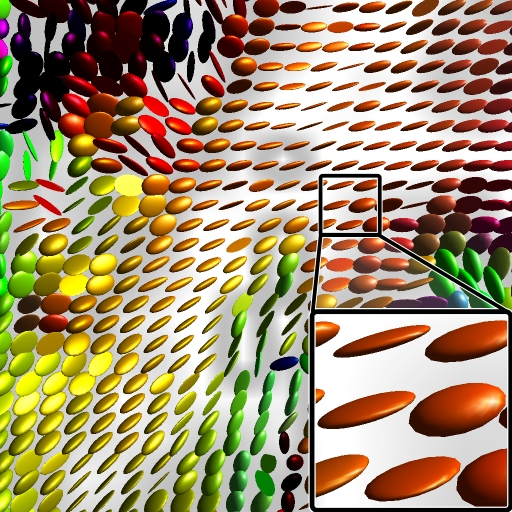
\includegraphics[width=0.3\linewidth]{figures/background/dti-glyph1.jpg}
		\label{fig:background:dti-glyph1}
	}
	\
	\subfloat[~Cuboid Glyphs.]{
		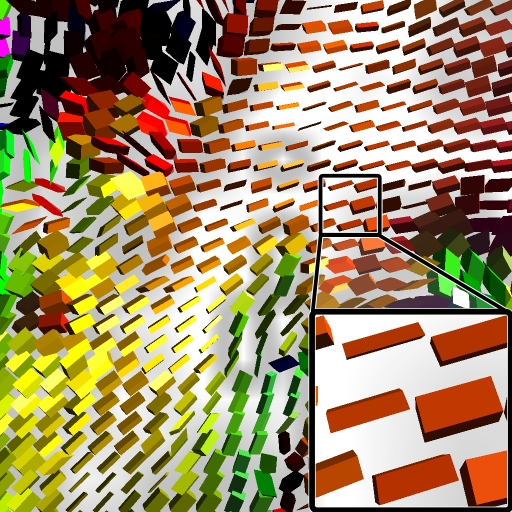
\includegraphics[width=0.3\linewidth]{figures/background/dti-glyph2.jpg}
		\label{fig:background:dti-glyph2}
	}
	\
	\subfloat[~Composed Glyphs.]{
		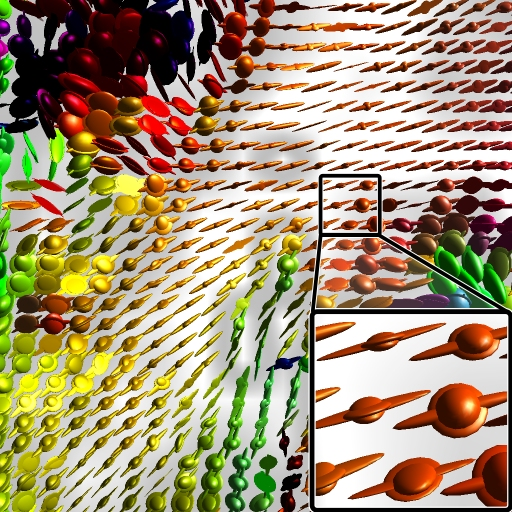
\includegraphics[width=0.3\linewidth]{figures/background/dti-glyph3.jpg}
		\label{fig:background:dti-glyph3}
	}
	\caption{
		Examples of different glyph visualization techniques for DTI data. Each image shows an axial slice through the corpus callosum of a human brain. 
		Besides the local information, the arrangement of the glyphs can also show some global features of the tensor field.
	}
	\label{fig:background:dti-glyphs}
\end{figure}


\subsubsection{Multi-modal Visualization}
Combining multiple imaging modalities is a powerful tool for clinicians since every modality exhibits certain strengths and weaknesses.
Functional imaging modalities such as PET for instance often have a very small resolution.
Putting them in context with an anatomical imaging modality such as CT or MR provides the clinician with a spatial reference so that functional hot spots can be associated with the corresponding anatomies.
Traditional techniques for multi-modal visualization are juxtaposition, image fusion (superimposition) and glyph techniques.
Fuchs and Hauser provide an overview over the state-of-art techniques for visualization of multivariate scientific data in \cite{Fuchs:2009:MultivariateSciVis}.

The juxtaposition of multiple images (i.e. showing them side by side) is the most straight-forward approach and requires the least amount of preprocessing. 
However, it also requires the highest amount of mental mapping by the observer, since they have to locate the correspondences between the images themselves.
In case the data sets are registered, linking techniques can facilitate this process -- for instance by always showing a slice of same position and orientation throughout all modalities \II.

Image fusion describes the embedding of multiple images into the same reference frame.
Unless the images are acquired from the same device in the same configuration, an initial registration process is required to align the images to each other.
In the subsequent visualization process the images are either first rendered individually and then blended together into the final image (suitable approach for 2D visualizations or geometry-based rendering techniques) or directly rendered together in a single pass (required for ray-casting volume rendering).
In any case, special care has to be taken to \SYN{carefully} adjust the transfer functions of each image to \SYN{match} the entire scene in order to avoid occlusion and ensure that the resulting image is still \SYN{readable}.
Different approaches have been proposed to make this process more user-friendly.
Haidacher et al. suggest to use a generic information-based technique to identify complementary information in two data sets and thereby reduce the parameter space \cite{Haidacher:2008:MultimodalVis}.
Focus-and-context techniques such as cutaways can further improve the understanding of the complex data and allow deep structures to be shown.
Beyer et al. present a fully integrated rendering system for neuro surgical planning supporting such cutaways and an arbitrary number of fused volumes and geometries \cite{Beyer:2007:MultimodalRendering}.
A recent approach also using illustrative visualization techniques is the work presented by Lawonn et al. focusing on fusing PET and CT scans \cite{Lawonn:2015:IlusstrativePetCt}.
\begin{figure}[ht]
	\centering
	\subfloat[~Multi-modal visualization for neuro surgery planning as shown in \cite{Beyer:2007:MultimodalRendering}.]{
		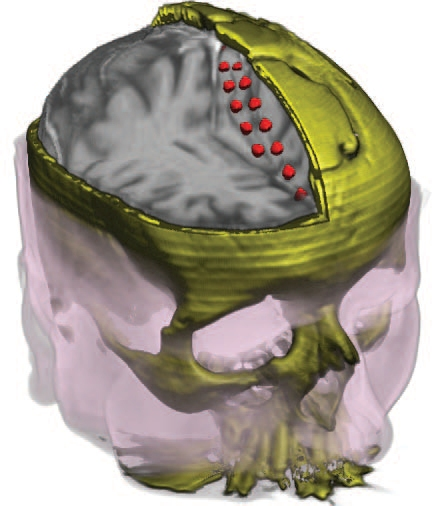
\includegraphics[height=4.75cm]{figures/background/beyer-multimodal1.jpg}
	}
	\quad
	\subfloat[~Multi-modal PET/CT visualization as shown in \cite{Lawonn:2015:IlusstrativePetCt}.]{
		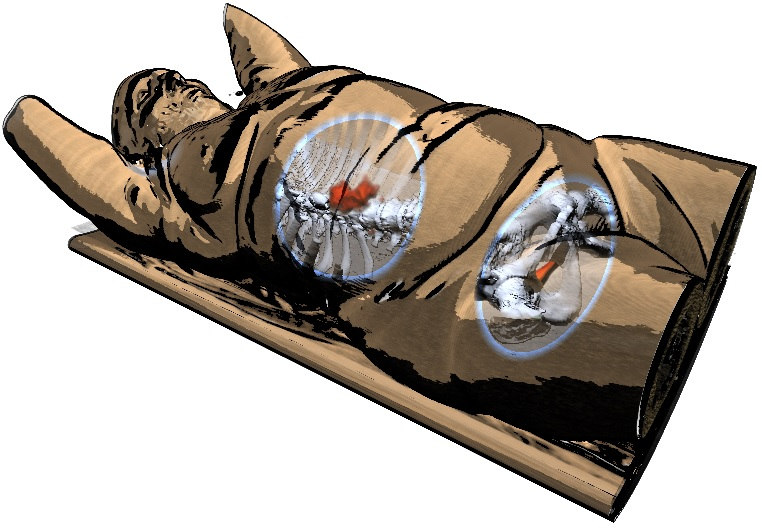
\includegraphics[height=4.75cm]{figures/background/lawonn-multimodal.jpg}
	}
	\caption{
		Examples for state-of-the-art multi-modal volume rendering using illustrative techniques such as cutaways and lenses.
	}
	\label{fig:background:multimodal}
\end{figure}

Glyph techniques are a very flexible way of visualizing multivariate data, where there are multiple output variables for each data element.
Their strength is the support of quantitative analysis of specific features in the data, in particular when used in hybrid visualizations that provide a spatial context.
Glyphs are simple polygonal objects with a fixed set of optical properties such as color, size, etc.
Besides classic glyphs such as arrows, ellipsoids or cuboids, which have already been mentioned in the previous section on high-dimensional medical data visualization, more advanced glyphs exists that allow to depict more measures through additional optical properties.
The supersphere, seamlessly interpolating between cube and sphere, allows to map one additional parameter to roundness.
Similarly, the supertorus allows to map two additional parameters to roundness and thickness as illustrated in Figure \ref{fig:background:superquadric-glyphs}.
\begin{figure}[ht]
	\centering
	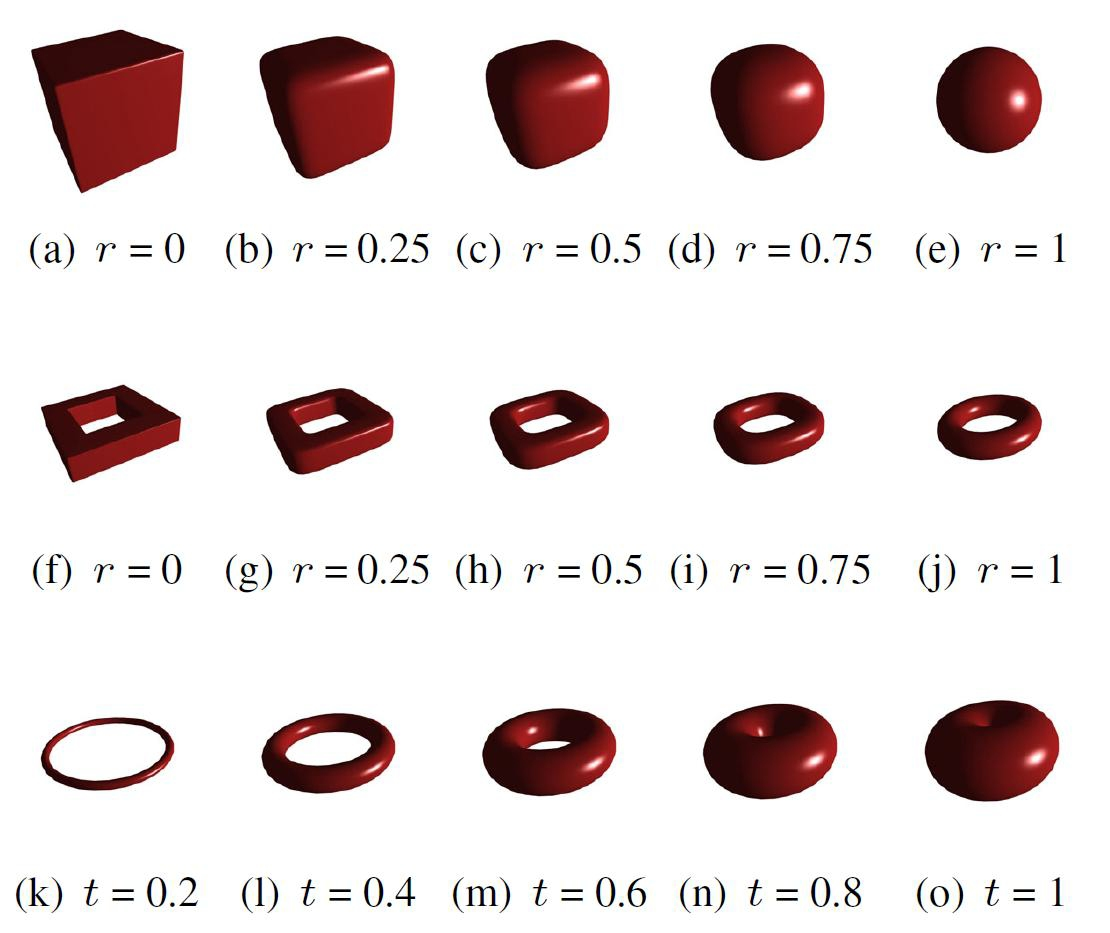
\includegraphics[width=0.75\linewidth]{figures/background/superquadric-glyphs.jpg}
	\caption{
		Illustration of the additional parameter space of the supersphere and supertorus glyphs.
		Both allow to map one parameter to the roundness.
		The supertorus has the additional property of thickness.
		Image from \cite{Ropinski:2007:Surfaceglyphs}.
	}
	\label{fig:background:superquadric-glyphs}
\end{figure}

While glyphs offer an effective means of visualizing highly multivariate data, their application and usage, particularly for 3D visualizations, is not straight-forward.
In \cite{Ropinski:2008:GlyphTaxonomy}, Ropinski and Preim define a taxonomy for glyphs based on the kind of visual information processing (e.g. pre-attentive vs. attentive processing; cf. Section \ref{sec:background:perception}) and derive usage guidelines for glyph-based medical visualization.
They argue that the glyph placement is crucial, since glyphs are usually placed onto the surface of the anatomy of interest in order to display additional information.
In such a setup, visual cluttering should be avoided and it must be ensured, that neither do the glyphs occlude each other nor do the glyphs occlude large parts of the anatomy.
Therefore, different glyph placement strategies have been proposed \cite{Ward:2002:GlyphPlacement}. 
\begin{figure}[ht]
	\centering
	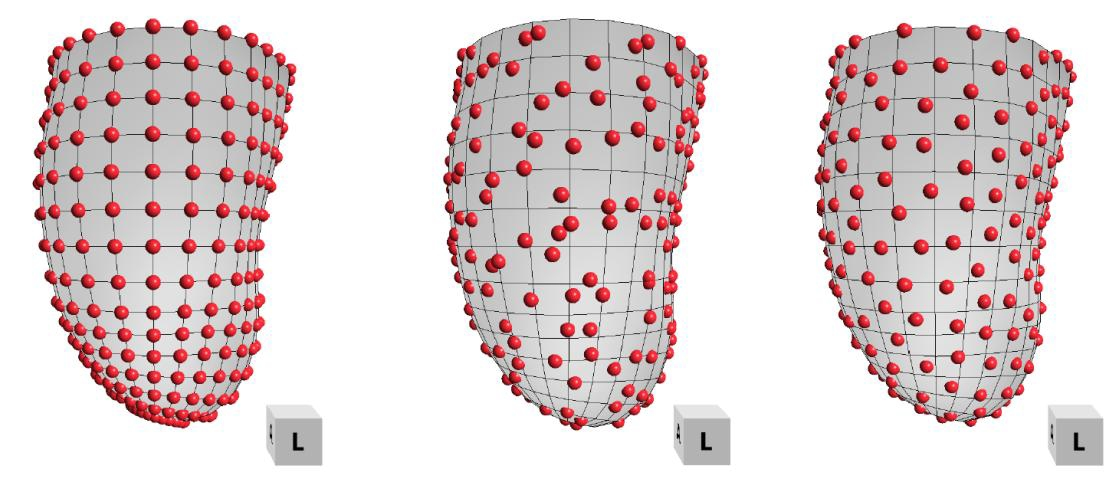
\includegraphics[width=0.75\linewidth]{figures/background/glyph-placement.jpg}
	\caption{
		Comparison of different glyph placement stategies.
		From left to right: regular grid, random distribution, random distribution with relaxation.
		Image from \cite{MeyerSpradow:2008:GlyphVis}.
	}
	\label{fig:background:glyph-placement}
\end{figure}
In general, a good glyph-based visualization ensures that the shapes are unambiguously perceivable and that unwanted glyph aggregations in image space due to bad placement is avoided.
The parameter mapping should visually emphasize important variables and thereby guide the user's focus of attention.
Furthermore, it should incorporate the semantics of the underlying data in order to facilitate the mental reconstruction of the information by the observer.
Good demonstrations of the power of such visualizations can be found in the works of Meyer-Spradow et al. \cite{MeyerSpradow:2008:GlyphVis} and Oeltze et al. \cite{Oeltze:2008:GlyphVis}.


\subsection{Ultrasound Visualization}
\label{sec:Background:UltrasoundVisualization}
%So far, there is not really that much scientific work on ultrasound visualization. Thus the things discussed here are rather basic and general. 
%Nevertheless, there should be a distinct section on US Vis as this is the main topic of this thesis.
The special nature of ultrasound images compared to traditional tomography modalities such as CT or MRI poses special challenges for visualization.
Since 2D images can be directly embedded into the rendering viewport, the display of 2D B-mode ultrasound is very straight-forward as the intensities are directly translated into brightness.
Additional information, such as Doppler or elastography ultrasound, is usually displayed through color overlays.
However, when moving towards 3D ultrasound imaging, traditional visualization techniques often yield unsatisfactory result and therefore require additional processing.
Birkeland et al. provide an in-depth overview over the ultrasound visualization pipeline in \cite{Birkeland:2012:UsVisPipeline}.

\subsubsection{Filtering}
While the characteristic speckle pattern provides important cues to clinicians when looking at 2D ultrasound images, the inhomogeneous intensity distribution leads to a very noisy appearance and unwanted occlusion in 3D visualizations.
Thus, advanced structure-preserving filtering is essential in order to get satisfactory results.
Traditional implementations employ median filtering or other non-linear methods based on wavelets, total variation or anisotropic diffusion. 
A comparison of their performance on ultrasound despeckling can be found in the the work by Michailovich and Tannenbaum \cite{Michailovich:2006:Despeckling}.
In a recent work, Soltészová et al. propose a streamline integration method along the direction of lowest variance \cite{Solteszova:2012:UsFiltering}.
Since it can be assumed that the anatomy structures are oriented in this direction, averaging the samples along the streamlines yields \SYN{good} results.
Exemplary results are shown in Figure \ref{fig:background:solteszova-filtering}.
\begin{figure}[ht]
	\centering
	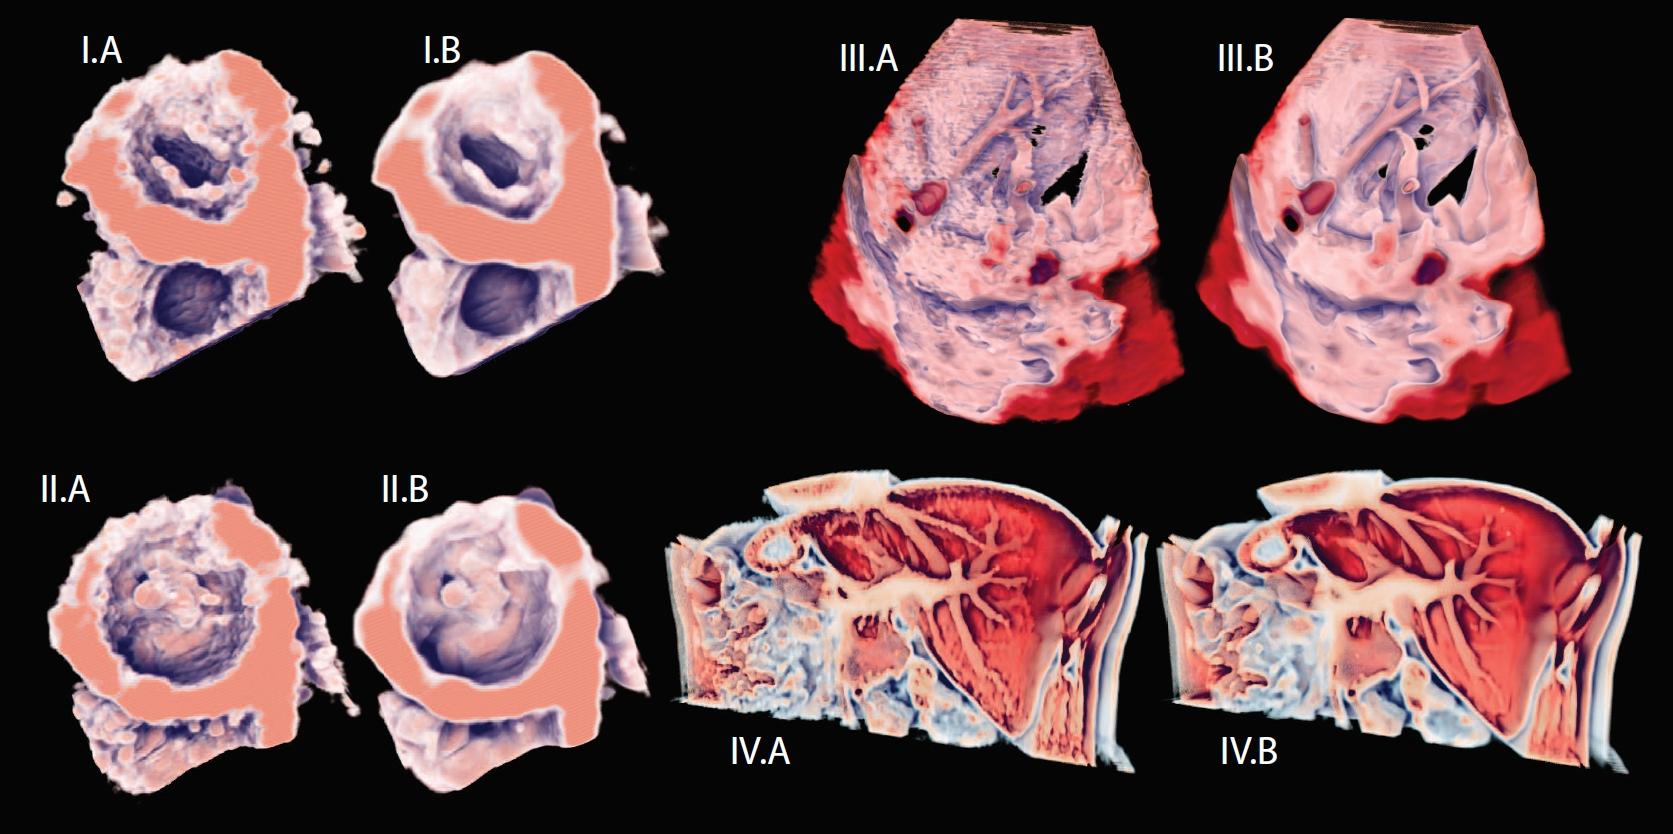
\includegraphics[width=0.75\linewidth]{figures/background/solteszova-filtering.jpg}
	\caption{
		Exemplary results of the lowest-variance-based filtering method of Soltészová et al. Image from \cite{Solteszova:2012:UsFiltering}.
	}
	\label{fig:background:solteszova-filtering}
\end{figure}

Since it is an essential feature that ultrasound imaging is real-time capable, the acceptable complexity of the filtering method is limited by the target frame rate.
Though the computational power of the today's hardware is constantly increasing and many filtering methods can be parallelized on GPUs, not all methods allow for an interactive processing of the incoming images.
To reduce the computational burden, Soltészová et al. propose a visibility-driven approach to the processing of streamed ultrasound volumes \cite{Solteszova:2014:VisibilityStreaming}.
After estimating the set of potentially visible voxels with respect to the current view point, they reduce the problem size by restricting the filtering process to those voxels and can thereby increase the performance.


\subsubsection{Classification}
Assigning optical properties such as color and opacity to ultrasound intensities for volume rendering poses various challenges as well.
Traditional classification methods are \SYN{hard} to apply due to the low dynamic range and the significant amount of noise.
Most importantly, B-mode ultrasound exhibits different intensities for the same tissue (cf. Section \ref{sec:background:imaging-modalities}).
This renders standard one-dimensional transfer function approaches \SYN{mostly useless} since the resulting images show low contrast and a high amount of occlusion.

One early method, specifically tackling these challenges for visualization, is the work of Sakas et al. \cite{Sakas:1995:UsVis}.
Fattal and Lischinski propose a variational approach based on the local value and gradient that performs filtering and opacity classification in a single unified process.
This allows them to extract smooth surfaces from 3D fetal ultrasound volumes \cite{Fattal:2001:VariationalClassification}.
Another challenge of ultrasound classification is the high \SYN{variability} of intensities between different images, which requires opacity transfer functions to be carefully optimized for each data set.
Therefore, Hönigmann et al. propose an automatic method to adjust the global opacity transfer function based on the intensity distribution along selected scanlines \cite{Honigmann:2003:AdaptiveOTF}.

\begin{figure}[ht]
	\centering
	\subfloat[~Real image acquired through a fetoscope.]{
		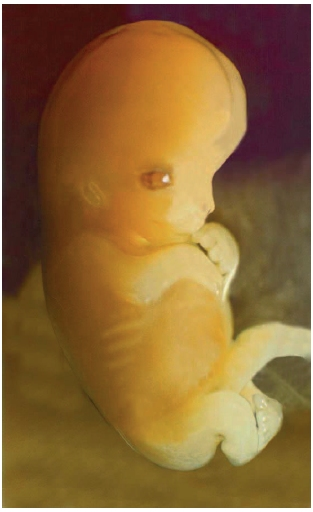
\includegraphics[height=6cm]{figures/background/varchola-fetoscope.jpg}
	}
	\quad
	\subfloat[~Fetoscopic rendering of a ultrasound volume.]{
		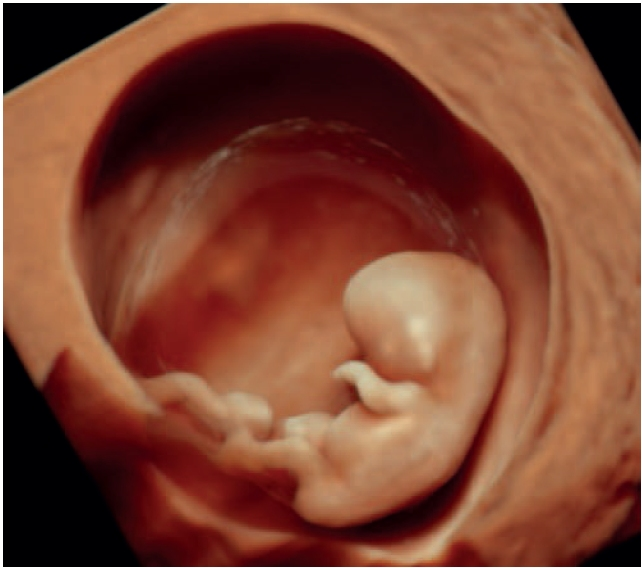
\includegraphics[height=6cm]{figures/background/varchola-rendering.jpg}
	}
	\caption[Comparison of an image acquired during fetoscopy with a fetoscopic rendering of 3D ultrasound.]{
		Tight integration of state-of-the algorithms allows for high-quality real-time fetal ultrasound imaging mimicking the appearance of fetoscopic imaging.
		Images from \cite{Varchola:2012:Fetoscopic}.
	}
	\label{fig:background:fetoscopic-rendering}
\end{figure}

By combining state-of-the-art algorithms throughout all steps of the volumetric ultrasound visualization pipeline, Andrej Varchola developed a fully integrated system allowing for high-quality renderings of prenatal ultrasound in real-time.
Advanced structure-preserving filtering, dynamic global illumination and realistic rendering of the human skin yield results of \SYN{astonishing} quality mimicking the appearance of fetoscopy images (cf. Figure \ref{fig:background:fetoscopic-rendering}) \cite{Varchola:2012:Fetoscopic}.
While the visual quality of the fetoscopic rendering is quite impressive, one has to keep in mind that prenatal ultrasound has a much better acoustic configuration compared to other anatomies since the fetus is surrounded by amniotic fluid exhibiting excellent transmission properties.
Thus, the results are not necessarily transferable to other ultrasound applications.

\section{Human Visual Perception}
\label{sec:background:perception}
%Explain why we should understand the human visual system in order to create better visualization.
The human visual system of perception and cognition is complex.
The eye serves as broadband channel into the mind since ca. 80\% of the environment is perceived visually \CN and roughly 50\% of the human brain deals with processing this visual input \CN.
Getting an understanding of how this works helps in designing better visualization since one can explain why a certain output is suitable for clinical practice and another is not.

%\subsection{Human Visual System}
%How does the human brain process visual input, pre-attentive processing, further perception phenomena
The human visual system perceives only a limited bandwidth of the light spectrum, \SYN{comprising light with a wavelength between $400$ and $700$ nm}, as initial sensation for the rods and cones in the retina.
After leaving the retina, neuronal signals pass through the optic nerve and optic tract to the visual cortex where they are initially processed in the primary visual receiving area (V1). 
From there they are forwarded along the dorsal pathway for object location and motion, as well as along the ventral pathway for object recognition and form representation \cite{Goldstein:2013:Perception}.

\subsection{Visual Attention}
However, what people actually see is not simply a translation of retinal stimuli but actually the result of the complex system of visual processing, which motivates the perception theory.
According to the feature integration theory, this cognitive process of visual processing can be divided into two stages.

It starts with the parallel processing of single features such as form, orientation, color and motion (\emph{preattentive stage}), and then continues sequentially with the combination of the features into 2D patterns, contours and object identification (\emph{focused attention stage}) \cite{Treisman:1985:PreattentiveProcessing}.
Preattentive processing applies to various features underlying a pop-out mechanism, which occurs prior to the conscious attention.
This salience is mostly independent of the number of distractors in feature search tasks, such as the one depicted in Figure \ref{fig:background:FeatureSearch}.
Conjunction searches, however, where a combination of multiple stimuli is \SYN{targeted} (cf. Figure \ref{fig:background:FeatureSearch}), can no longer be performed preattentively since the features have to be combined in the focused attention stage.
This visual search has to be performed by sequentially by looking at each target and thus requires significantly more time (cf. Figure \ref{fig:background:ResponseTimes}).
\TODO{Conclusion for this thesis.}



\subsection{Perceptual Organization}
\TODO{rewrite in your own words}
%Basic principles of Gestalt theory and the Gestalt Laws as in Timo's lecture slides.
Perceptual organization is the process by which elements in the environment become perceptually grouped to create our perception of objects.
During this process, incoming stimulation is organized into coherent units, such as objects.
The process of perceptual organization involves two components, \emph{segregation} and \emph{grouping} \cite{Peterson:2013:PerceptualOrganization}.
Grouping is the process by which visual events are put together into units or objects.
THe process of grouping works in conjunction with segregation, which is the process of separating one area or object from another. \III{Image with skyline, illustrating segregation and grouping}

The cause of this process of grouping visual elements into objects can be explained by the Gestalt theory \CN.
In the early 1900s, the Gestalt psychologists discovered/defined a set of organizing principles, which determine how elements in a scene become grouped together.
\begin{my_list_desc}
	\item[Good Continuation]
		Points that when connected result in straight or smoothly curving lines are seen as belonging together, and the lines tend to be seen in such a way as to follow the smoothest path.
		Objects that are partially covered by other objects are seen as continuing behind the covering object.
	
	\item[Pragnanz]
		Every stimulus pattern is seen in such a way that the resulting structure is as simple as possible.
	
	\item[Similarity]
		Similar things appear to be grouped together.
	
	\item[Proximity]
		Things that are near each other appear to be grouped together.
	
	\item[Commopn Fate]
		Things that are moving in the same direction appear to be grouped together.
	
	\item[Common Region]
		Elements that are within the same region of space appear to be grouped together.
	
	\item[Uniform Connectedness]
		A connected region of the same visual properties, such as lightness, color, texture, or motion, is perceived as a single unit.
\end{my_list_desc}
These principles are extended by the principles of figure and ground, which are responsible for perceptual segregation, i.e. the identification of foreground object and background.

Furthermore, our knowledge of regularities in the environment help us perceive.
\emph{Physical regularities} are regularly occuring physical properties of the environment. 
A very strong one is the light-from-above assumption \cite{Kleffner:1992:ShapeFromShading}.
Since most light in our environment comes from above, we intuitively perceive \II a as indentations in the sand while \II b look like mounds of sand, even though it is the same image just turned upside down.
Other examples of physical regularities are the stronger presence of vertical and horizontal orientations than oblique (angled) orientations \cite{Coppola:1998:UnequalRepresentations}, as well as that objects in the environment often have homogeneous colors and nearby objects have different colors.
\emph{Semantic regularities} helps us identifying objects in a scene with a certain meaning.
It allows to identify ambiguous stimuli as objects, which we would expect in the context of the scene \cite{Oliva:2007:RoleOfContext}.



\subsection{Perceiving Depth and Size}
\TODO{rewrite in your own words}
\TODO{Depth percerption is inportant, blablabla}
The perception of depth cues can be categorized into three groups:
\begin{my_list_num}
	\item
		\emph{Oculomotor} cues based on the ability to sense the position of our eyes and the tension on our eye muscles.
	\item
		\emph{Monocular} cues that work with one eye.
	\item
		\emph{Binocular} cues that depend on two eyes.
\end{my_list_num}

\paragraph{Oculomotor Cues}
The oculomotor cues are created by convergence, the inward movement of the eyes that occurfs when we look at nearby objects, and accomodation, the cahnge in shape of the lens that occurs when we focus on objects at various distances.
The idea behind these cues is that we can feel the inward movement of the eyes when the eyes converge to look at nearby objects.
Convergence and accomodation indicate when an objects is close and are useful up to a distance of about arm's length, with convergence being the more effective of the two \cite{Mon-Williams:1999:ExtraretinalContribution, Tresilian:1999:Vergence}.

\paragraph{Monocular Cues}
Monocular cues work with only one eye and can be grouped into pictorial cues, which can be depicted in a single picture and motion-produced cues.
The larger group is the former one \III{Example image we can refer to}:
\begin{my_list_desc}
	\item[Occlusion]
		Occlusion occurs when one object hides or partially hides another from view.
		It provides only a relative measure of depth.
		Thus one perceives that the occluded object is farther away, but not by how much.
	
	\item[Relative Height]
		Objects with their bases closer to the horizon are usually seen as being more distant.
		This means that being higher in the field of view causes objects on the ground to appear farther away, whereas being lower in the field of view causes objects in the sky to appear farther away.
	
	\item[Relative Size]
		When two objects are of equal size, the one that is farther away will take up less of your field of view than the one that is closer.
	
	\item[Perspective Convergence]
		When you look down parallel railroad tracks that appear to converge in the distance, you are experience PC.
	
	\item[Atmospheric Perspective]
		Atmospheric perspective occurs when distant objects appear less sharp than near objects and often have a slight blue tint.
		The farther away an object is, the more air and particles (dust, water droplets, airborne pollution) we have to look through, making objects that are farther away look less sharp and bluer than close objects.
	
	\item[Texture Gradient]
		Elements that are equally spaced in a scene appear to be more closely packed as distance increases.
	
	\item[Shadows]
		Shadows -- decreases in light intensity caused by the blockage of light -- can provide information regarding locations of these objects.
	
	\item[]
		
	
\end{my_list_desc}

All of the cues we have described so far work if the observer is stationary. But once we start moving, new cues emerge that further enhance our perception of depth:
\begin{my_list_desc}
	\item[Motion Parallax]
		Motion parallax occurs when, as we move, nearby objects appear to glide rapidly past us, but more distant objects appear to move more slowly.
		Motion parallax is one of the most important sources of depth information for many animals. 
		The information provided by motion parallax has been used to enable human-designed mechanical robots to determine how far they are from obstacles as they navigate through the environment.
		It is also widely used to create an impression of depth in cartoons and video games.
	
	\item[Deletion and Accretion]
		As an observer moves sideways, some things become covered, and others become uncovered.
\end{my_list_desc}


\paragraph{Binocular Cues}
Although it is possible to use the above monocular cues to see depth, there is something qualitatively different about the depth perception experienced when using both eyes.
Two-eyed depth perception, called stereoscopic vision, involves mechanisms that take into account differences in the images formed on the left and right eyes.

An impressive description of how much stereoscopic vision qualitatively differs from monocular depth perception can be found in the story of Susan Barry \cite{Barry:2009:FixingMyGaze}.
Originally being cross-eyed \TODO{strabismus}, her visual system suppressed the vision in one of the eyes to avoid a double vision.
Thus, she saw the world with only one eye at a time.
Although her perception of depth was achieved through monocular cues, she was able to get along quite well and could participate in daily activity such as driving a car and sports.
This was until she embarked on an intensive course of training with a developmental optometrist, and one day, after learning to align her eyes, she suddenly saw the steering wheel of her car popping out from the dashboard.
After having lived in a flat world for fifty years, she felt this leap into three-dimensionality as a revelation.

Binocular disparity, the differences in the images on the left and right retinas, is the basis of the stereoscopic vision.
This effect appears due to the eyes' horizontal separation yielding to an absolute and relative disparity, where the images of objects at different depths fall on non-corresponding points in the two retinas.
Though this disparity is rather a geometrical than a perceptual effect, it is the basis for the stereopsis, since the angle of disparity allows to estimate the relative depths ob multiple objects to each other.


\subsection{Color Perception}
\label{sec:background:colorperception}
%color perception, usage of color maps
The perception of color is a psychophyiscal process.
While the physical properties of light, such as wavelengths, spectral distribution and intensity are given by the environment, the psychological and perceptual process in the human visual system transforms these sensations after they have been registered in the retina.
Color can be \SYN{generalized} into the three perceptual dimensions of hue, saturation and intensity, having a non-linear relation to the physical properties \cite{Goldstein:2013:Perception}.
While the hue (i.e. the color of the rainbow such as blue, green, red, yellow) corresponds to the predominant wavelengths, it's saturation (i.e. chromacity/paleness) corresponds to the spectral distribution of the incoming light.
Finally, the color intensity (i.e. lightness/darkness) is related to the amount of light entering the retina.

When performing visualization, one should choose the applied colors carefully, as they have individual perceptual effects.
For instance, short wavelengths are usually perceived as being farther away than long wavelengths due to the lens of the eye is refracting them at different angles \cite{Steenblik:1987:Chromadepth}.
This phenomenon was exploited by the pseudo-chromadepth technique of Ropinski et al. and illustrated in Figure \ref{fig:background:ropinski-angio-depth}.
It provides an improved depth perception in monocular angiography images by using a gradient color map running from red (long wavelength, close) to blue (short wavelength, far) \cite{Ropinski:2006:Chromadepth}.

\begin{figure}[ht]
	\centering
	\subfloat[~No color coding of depth]{
		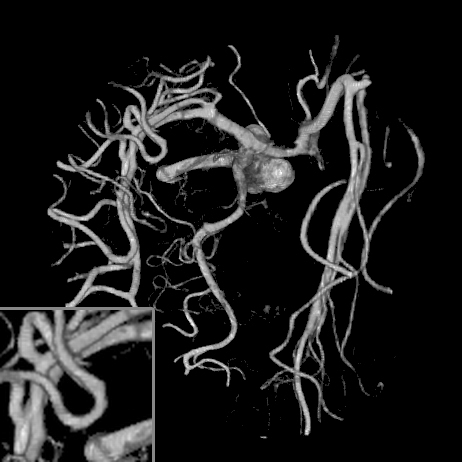
\includegraphics[width=0.3\linewidth]{figures/background/ropinski_standard.jpg}
	}
	\subfloat[~Chromadepth]{
		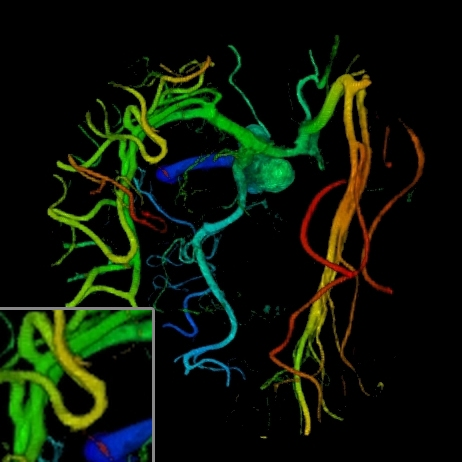
\includegraphics[width=0.3\linewidth]{figures/background/ropinski_chromadepth.jpg}
	}
	\subfloat[~Pseudo-chromadepth]{
		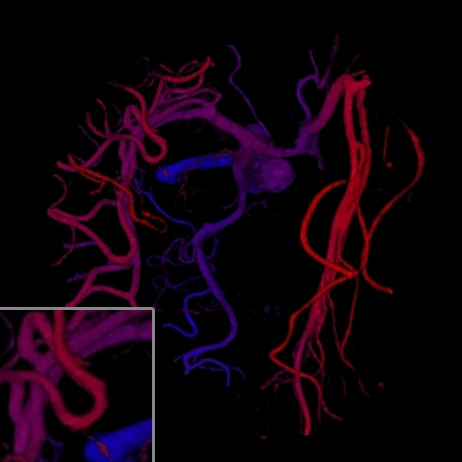
\includegraphics[width=0.3\linewidth]{figures/background/ropinski_pseudochromadepth.jpg}
	}
	\caption{
		Illustration of chromadepth and pseudo-chromadepth coding of depth in angiography images as shown in \cite{Ropinski:2006:Chromadepth}.
		Compared to the (a) and (b), image (c) provides the observer with a much better perception of relative depth just through the use of color mapping. 
	}
	\label{fig:background:ropinski-angio-depth}
\end{figure}

One very controversial topic in the visualization community still is usage of the rainbow color map for depicting numeric data.
Perceptual science argues that it has the two major flaws of missing ordering (no intuitive ordering of the main hues) as well as misleading banding effects \cite{Borland:2007:RainbowColormap}.
Nevertheless, the rainbow color map is still used very often in many scientific visualizations, which may be due to it being the default setting in many visualization tools, a lack of alternatives or scientists simply being used to reading such visualizations.

However, general guidelines exist for choosing good color tables with respect to the data type (cf. Section \ref{sec:Background:DataCharacteristics}) \cite{Borland:2007:RainbowColormap, Treinish:2009:Should}.
For nominal data, one should choose a selection of distinct colors.
High frequency ordinal data can be well represented with a luminance contrast color map such as the heated body scale.
When applying color mapping to surfaces, one should use an isoluminant scheme to preserve the perceived shape.
Finally, diverging color maps \cite{Moreland:2009:DivergingCM} provide an excellent means for showing interval and ratio data on two-ended scales.


\section{Evaluation of Visualization Methods}
%This was also once a comment of Nassir that I should discuss in my thesis how one can evaluate visualization techniques. 
%A starting point for this section could be the IEEEVis'14 workshop on exactly this topic.
The evaluation of scientific research can usually be divided into two groups: qualitative and quantitative evaluation.
While quantitative methods focus on the systematic empirical investigation and target \SYN{hard} statistical, mathematical or computational results, qualitative methods focus more on gathering knowledge on how and why something works in order to better understand the results.
Traditionally, research on visualization is rather hard to evaluate quantitatively since it is difficult to quantify how good a novel visualization technique is in comparison to the state of art due to perception being a very subjective \SYN{thing} and the resulting high subject-interrelatedness.
Thus, qualitative evaluation methods such as expert feedback or detailed analysis of case studies play an important role.
Nevertheless, quantitative evaluation methods are applicable if they are executed correctly.
This section discusses the different approaches of evaluation on visualization methods.

There exists a plethora of different validation methods. The following list is inspired from \cite{Munzner:2008:InfoVis} and should just \SYN{act} as overview over the possibilities.
\begin{my_list_item}
	\item Implementation performance, algorithm complexity analysis
	\item Quantitative metrics on domain-specific tasks, image quality, etc.
	\item Qualitative discussion of result pictures
	\item Case studies, user anecdotes (insights found)
	\item User studies on usability, intuitiveness, appreciation, etc.
	\item Design justification from task analysis
	\item Visual encoding justification from theoretical principles
\end{my_list_item}
However, deciding on how and when to apply these methods is not straight-forward since each of them targets specific aspects of visualization design.

Since many visualization techniques are rather application specific, task-dependent evaluation of design choices is a frequently used approach \cite{Lam:2012:EmpiricalStudies}.
This is particularly the case for medical visualization.
Tasks are an essential concept in order to provide a motivation and goal for medical visualization techniques as they are targeted to support the clinician during their work and with their decisions and therefore often specifically tailored to certain activities.
However, the term \emph{task} is often used ambiguously within the visualization community, as for instance they can be formulated very open-ended (e.g. ``find anomalies in the anatomy'') or specific (e.g. ``determine the diameter of aneurysm'').
Rind et al. therefore propose a three-dimensional conceptual space of user tasks in visualization and classify them by abstraction (concrete/abstract), composition (high-level/low-level) and perspective (why/how), which would make task-based evaluation easier comparable \cite{Rind:2014:Tasks}.

There have been different approaches towards generalizing the process of visualization evaluation, providing a wide range of methods and guidelines on how to apply them \cite{Kerren:2008:EvaluatingInformationVisualization, Plaisant:2004:ChallengeEvaluation}.
Tamara Munzner proposes a four-level hierarchical model (cf. Figure \ref{fig:background:munzner-nestedmodel1}) of visualization creation providing a framework on what methodology is appropriate for each of its levels.
Based on this model, she identifies possible threats for each level and derives applicable methods for validation (cf. Figure \ref{fig:background:munzner-nestedmodel2}) \cite{Munzner:2009:NestedModel}.
Though her work is focused on information visualization, her findings are certainly also applicable to the field of medical visualization.

Another approach to provide an all-encompassing evaluation model is presented by John Stasko who proposed value-driven evaluation of visualizations.
He \SYN{claims, suggests} that the value of a visualization is composed by four components and defines it as the sum of \cite{Stasko:2014:ValueDrivenEvaluation}:
\begin{my_list_item}
	\item The visualization's ability to minimize the total time needed to answer domain specific questions.
	\item The visualization's ability to spur questions and insight on the data.
	\item The visualization's ability to provide an overall essence of the data.
	\item The visualization's ability to generate confidence, knowledge, and trust about the data.
\end{my_list_item}

In the recent past, there have been some \SYN{attempts} to introduce new evaluation methods by adopting techniques from other fields.
Product reaction cards were originally proposed by Benedek and Miner \cite{Benedek:2003:Desirability} and provide a way to collect feedback on user experience orthogonal to traditional Likert scales, where the user rates the system on a pre-defined set questions on a fixed scale.
Instead, the user chooses from a set of cards, each containing an adjective, those that best reflect their experience.
Since the set contains both positive and negative cards, the selection allows for an elaborate analysis of the feedback \cite{Barnum:2010:MoreThanAFeeling, Mercun:2014:ReactionCards}.
Blaha et al. propose to build a recommender system out of user studies by conducting them in a structured manner.
This allows to apply machine learning techniques to their results, which then can lead to new insight on the relationships between the experimental data and metrics on the visualized data itself \cite{Blaha:2014:RecommenderSystem}.
Some time, such machine learning techniques might be capable of providing the visualization community with the goal \SYN{they long aimed for, yet did not reach so far}:
A formal perceptual model that allows to quantify the value of a visualization technique.

